% \mhb{\alpha}
\section{Introduction}

%\paragraph{Motivation}

Simultaneously imaging large populations of neurons using calcium sensors is becoming increasingly popular \cite{ImagingManual}, both \emph{in vitro} \cite{SmettersYuste99, IkegayaYuste04} and \emph{in vivo} \cite{NagayamaChen07, GobelHelmchen07, LuoSvoboda08}, and will likely continue as the signal-to-noise-ratio (SNR) of genetic sensors continues to improve \cite{GaraschukKonnerth07, MankGriesbeck08b, WallaceHasan08}.  Whereas the data from these experiments are movies of time-varying fluorescence traces, the desired signal consists of spike trains of the observable neurons. Unfortunately, finding the most likely spike train is a challenging computational task, due to limitations of the SNR and temporal resolution, unknown parameters, and computational intractability. %One is therefore effectively forced to find an approximately most likely spike train, or hope that the inferred spike train is indeed most likely. 

A number of groups have therefore proposed algorithms to infer spike trains from calcium fluorescence data using very different approaches.  Early approaches simply thresholded $dF/F$ (e.g., \cite{Schwartz98,Mao01}) to obtain ``event onset times.''  More recently, Greenberg et al \cite{GreenbergKerr08} developed a  template matching algorithm to identify individual spikes. %, which performed well on their data, but is not particularly computationally efficient
Holekamp et al \cite{HolekampHoly08} then applied an optimal linear deconvolution (i.e., the Wiener filter) to the fluorescence data.  This approach is natural from a signal processing standpoint, but does not utilize the knowledge that spikes are always positive.  Sasaki et al \cite{SasakiIkegaya08} proposed using machine learning techniques to build a nonlinear supervised classifier, requiring many hundreds of examples of joint electrophysiological and imaging data to ``train'' the algorithm to learn what effect spikes have on fluorescence.  Vogelstein et al \cite{VogelsteinPaninski09} proposed a biophysical model-based sequential Monte Carlo method to efficiently estimate the probability of a spike in each image frame, given the entire fluorescence time-series.  While effective, that approach is not suitable for online analyses of populations of neurons, as the computations run in about real-time per neuron (ie, analyzing one minute of data requires about one minute of computational time on a standard laptop computer).

In the present work, a simple model is proposed relating spiking activity to fluorescence traces. Unfortunately, inferring the most likely spike train given this model is computationally intractable.  Making some reasonable approximations leads to an algorithm that infers the approximately most likely spike train, given the fluorescence data.  This algorithm has a few particularly noteworthy features, relative to other approaches.  First, spikes are assumed to be positive.  This assumption often improves filtering results when the underlying signal has this property \cite{PortugalVicente94, MarkhamConchello99, LeeSeung99, LLS04, OGradyPearlmutter06, HuysPaninski06, Cunningham08, PaninskiWu09}.  Second, the algorithm is fast: it can process a calcium trace from 50,000 images in about one second on a standard laptop computer. In fact, filtering the signals for an entire population of over 100 neurons runs faster than real-time. This speed facilitates using this filter online, as observations are being collected. In addition to these two features, the model may be generalized in a number of ways, including incorporating spatial filtering of the raw movie, which can improve effective SNR. The utility of the proposed filter is demonstrated on several biological data-sets, suggesting that this algorithm is a powerful and robust tool for online spike train inference.  The code (which is a simple Matlab script) is available from \url{http://wwww.optophysiology.org}.







\section{Methods} \label{sec:methods}

%As mentioned above, starting with an \emph{in vitro} experiment, for which the SNR is relatively high, an appropriate generative model can be built (section \ref{sec:model}).  Given this model, a goal can be formalized (section \ref{sec:goal}).  And given this goal, an approximately optimal inference algorithm is derived (section \ref{sec:inf}) .  This algorithm depends on a number of unknown parameters, which can be estimated directly from the fluorescence observations (section \ref{sec:learn}).  The effective signal-to-noise ratio (SNR) of the fluorescence trace can be potentially improved by spatially filtering the movie (section \ref{sec:methods:spatial}), even when multiple neurons are within a region-of-interest (ROI) (section \ref{sec:methods:overlapping}).  


\subsection{Data driven generative model} \label{sec:model}

Figure \ref{fig:in_vitro_ex} shows data from a typical \emph{in vitro} epifluorescence experiment (see section \ref{sec:exp} for data collection details).  The top panel shows the mean frame of this movie, including 3 neurons, two of which are patched.  To build the model, the pixels within a region-of-interest (ROI) are selected (white circle).  Given the ROI, all the pixel intensities of each frame can be averaged, to get a one-dimensional fluorescence time-series, as shown in the bottom left panel (black line).  By patching onto this neuron, the spike train can also be directly observed (black bars). Previous work suggests that this fluorescence signal might be well characterized by convolving the spike train with an exponential, and adding noise \cite{ImagingManual}.  This model is confirmed by convolving the true spike train with an exponential (gray line, bottom left panel), and then looking at the distribution of the residuals.  The bottom right panel shows a histogram of the residuals (dashed line), and the best fit Gaussian distribution (solid line).


\begin{figure}[h!]
\centering 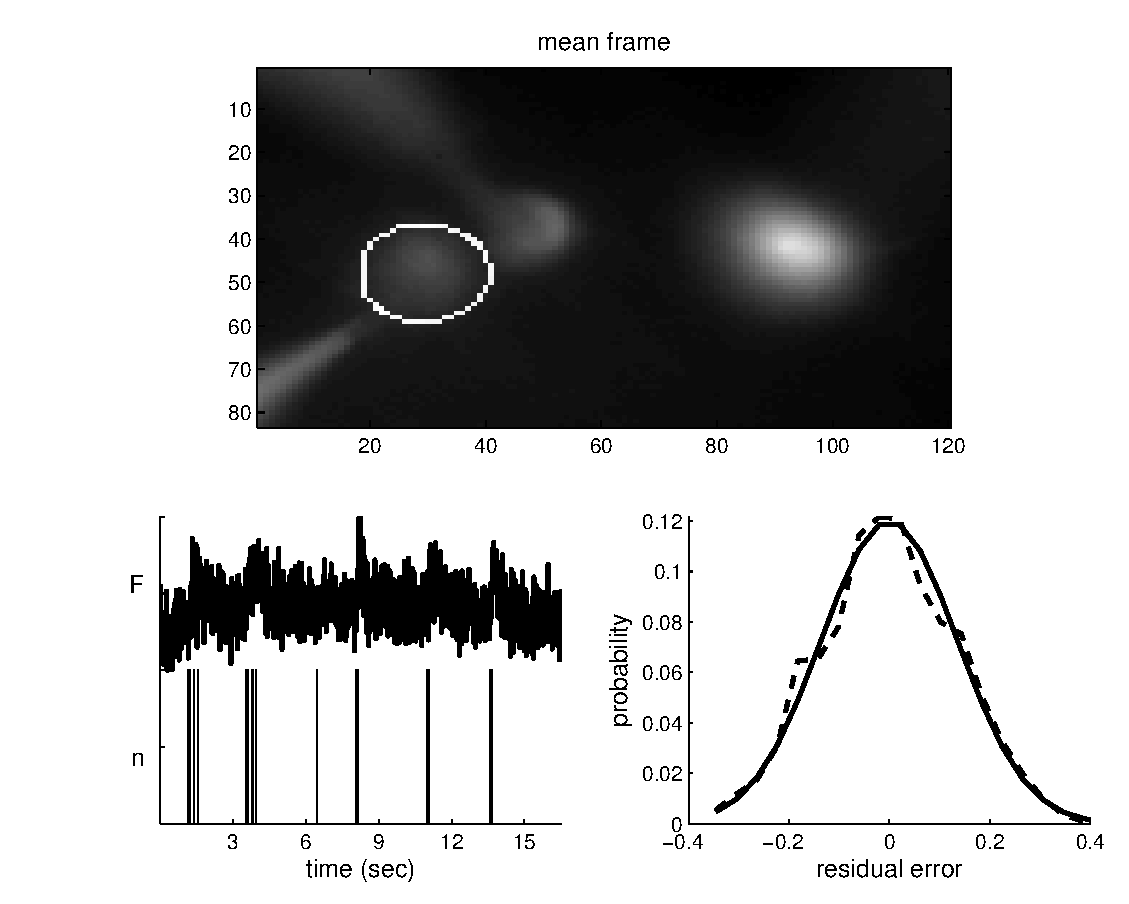
\includegraphics[width=.9\linewidth]{/Users/joshyv/Research/oopsi/fast-oopsi/figs/in_vitro_ex}
\caption[data-based model]{Typical \emph{in vitro} data suggest that a reasonable first order model may be constructed by convolving the spike train with an exponential and adding Gaussian noise. Top panel: the average (over frames) of a typical field-of-view.  Bottom left: true spike train recorded via a patch electrode (black bars), convolved with an exponential (gray line), superimposed on the fluorescence trace (OGB-1; black line).  While the spike train and fluorescence trace are measured data, the calcium is not directly measured, but rather, inferred.  Bottom right: a histogram of the residual error between the gray and black lines from the bottom left panel (dashed line), and the best fit Gaussian (solid line). Note that the Gaussian model provides a good fit for the residuals here.} \label{fig:in_vitro_ex}
\end{figure}

The above observations may be formalized as follows. Assume there is a one-dimensional fluorescence trace, $\mb{F}$ (throughout this text $\mb{X}$ indicates the vector $[X_1, \ldots, X_T]$, where $T$ is the index of the final frame), from a neuron.  At time $t$, the fluorescence measurement $F_t$ is a linear-Gaussian function of the intracellular calcium concentration at that time, $\Ca_t$:
\begin{align} \label{eq:F}
F_t &= \alpha \Ca_t + \beta + \sig \varepsilon_t, \qquad \varepsilon_t \overset{iid}{\sim} \mc{N}(0,1).
\end{align}
\noindent The scale, $\alpha$, absorbs all experimental variables impacting the scale of the signal, including the number of sensors within the cell, photons per calcium ion, amplification of the imaging system, etc.  Similarly, the offset, $\beta$, absorbs the baseline calcium concentration of the cell, background fluorescence of the fluorophore, imaging system offset, etc.  The standard deviation, $\sig$, results from calcium fluctuations independent of spiking activity, fluorescence fluctuations independent of calcium, and imaging noise. The noise at each time, $\varepsilon_t$, is independently and identically distributed according to a standard normal distribution (ie, Gaussian with zero mean and unit variance), as indicated by the notation $\overset{iid}{\sim}\mc{N}(0,1)$. 

Then, assuming that the intracellular calcium concentration, $\Ca_t$, jumps by $A$ $\mu$M after each spike, and subsequently decays back down to $C_b$ $\mu$M with time constant $\tau$ sec, one can write:
\begin{align} \label{eq:C1}
\Ca_{t+1} = (1- \Del/\tau ) \Ca_t + (\Del/\tau) C_b + A n_t
\end{align}
\noindent where $\Del$ is the time step size --- which is the frame duration, or $1/$(frame rate) --- and $n_t$ indicates the number of times the neuron spiked in frame $t$. %, and $\gam=1-\Del/\tau$. \footnote{This follows from writing \eqref{eq:C} as $\tau \frac{C_t - C_{t-1}}{\Del} = -C_{t-1} + n_t$.} 
Note that because $\Ca_t$ and $F_t$ are linearly related to one another, the fluorescence scale, $\alpha$, and calcium scale, $A$, are not identifiable.  In other words, either can be set to unity without loss of generality, as the other can absorb the scale entirely. Similarly, the fluorescence offset, $\beta$, and calcium baseline, $C_b$ are not identifiable, so either can be set to zero without loss of generality.  Finally, letting $\gam=(1-\Del/\tau)$, Eq.~\eqref{eq:C1} can be rewritten replacing $\Ca_t$ with its non-dimensionalized counterpart, $C_t$: 
\begin{align} \label{eq:C2}
	 C_t =\gam C_{t-1} + n_t.
\end{align} 
\noindent Note that $C_t$ does not refer to absolute intracellular concentration of calcium, but rather, a relative measure (see \cite{VogelsteinPaninski09} for a more general model).  The gray line in the bottom left panel of Figure \ref{fig:in_vitro_ex} corresponds to the putative $\mb{C}$ of the observed neuron.  

To complete the ``generative model'' (ie, a model from which simulations can be generated), the distribution from which spikes are sampled must be defined.  Perhaps the simplest first order description of spike trains is that at each time, spikes are sampled according to a Poisson distribution with some rate:
\begin{align} \label{eq:n}
	n_t \overset{iid}{\sim} \text{Poisson}(\lam \Del)
\end{align}
\noindent where $\lam \Del$ is the expected firing rate per bin, and $\Del$ is included to ensure that the expected firing rate is independent of the frame rate.  Thus, Eqs.~\eqref{eq:F}, \eqref{eq:C2}, and \eqref{eq:n} complete the generative model.  






\subsection{Goal} \label{sec:goal}

Given the above model, the goal is to find the \emph{maximum a posteriori} (MAP) spike train, i.e.,  the most likely spike train, $\mhb{n}$,  given the fluorescence measurements, $\mb{F}$:
\begin{align} \label{eq:nhat1} 
\mhb{n} &=  \anx P[\mb{n} | \mb{F}], 
\end{align}
\noindent where $P[\mb{n} | \mb{F}]$ is the posterior probability of a spike train, $\mb{n}$, given the fluorescent trace, $\mb{F}$, and $n_t$ is constrained to be an integer, $\mathbb{N}_0=\{0,1,2,\ldots\}$, because of the above assumed Poisson distribution.  From Bayes' rule, the posterior can be rewritten:
\begin{align} \label{eq:bayes}
P[\mb{n} | \mb{F}] = \frac{P[\mb{n}, \mb{F}]}{P[\mb{F}]} = \frac{1}{P[\mb{F}]} P[\mb{F} | \mb{n}] P[\mb{n}],
\end{align}
\noindent where $P[\mb{F}]$ is the evidence of the data, $P[\mb{F} | \mb{n}]$ is the likelihood of observing a particular fluorescence trace $\mb{F}$, given the spike train $\mb{n}$, and $P[\mb{n}]$ is the prior probability of a spike train.  Plugging the far right-hand-side of Eq.~\eqref{eq:bayes} into Eq.~\eqref{eq:nhat1}, yields:
\begin{align} \label{eq:nhat2} 
\mhb{n} &=  \anx \frac{1}{P[\mb{F}]} P[\mb{F} | \mb{n}] P[\mb{n}] =  \anx  P[\mb{F} | \mb{n}] P[\mb{n}],
\end{align}
\noindent where the second equality follows because $P[\mb{F}]$ merely scales the results, but does not change the relative quality of any particular spike train.  Note that the prior $P[\mb{n}]$ acts as a regularizing term, potentially imposing sparseness or smoothness, depending on the assumed distribution \cite{WuGallant06,Seeger08}. Both $P[\mb{F} | \mb{n}]$ and $P[\mb{n}]$ are available from the above model:
\begin{subequations} \label{eq:post1}
\begin{align}
P[\mb{F} | \mb{n}]&= P[\mb{F} | \mb{C}] 	= \prod_{t=1}^T P[F_t | C_t], \label{eq:lik1} \\ 
P[\mb{n}] 		&= \prod_{t=1}^T P[n_t], \label{eq:prior1}
\end{align}
\end{subequations}
\noindent where the first equality in Eq.~\eqref{eq:lik1} follows because $\mb{C}$ is deterministic given $\mb{n}$, and the second equality follows from Eq.~\eqref{eq:F}. Further, Eq.~\eqref{eq:prior1} follows from the Poisson process assumption, Eq.~\eqref{eq:n}.  Both $P[F_t | C_t]$ and $P[n_t]$ can be written explicitly:
\begin{subequations} \label{eq:post2}
\begin{align}
P[F_t | C_t] &= \mc{N}(\alpha C_t+\beta,\sig^2), \label{eq:lik2} \\
P[n_t] &= \text{Poisson}(\lam \Del), \label{eq:prior2} 
\end{align}
\end{subequations}
%\noindent where $\mc{N}(x;\mu,\sig^2)$ indicates $x$ has a Gaussian distribution with mean $\mu$ and variance $\sig^2$ and Poisson$(x;r)$ indicates that $x$ has a Poisson distribution with rate $r$, and 
where both equations follow from the above model, and the Poisson distribution acts as a sparse prior.  Now, plugging Eq.~\eqref{eq:post2} back into \eqref{eq:post1}, and plugging that result into Eq.~\eqref{eq:nhat2}, yields:
\begin{subequations}  \label{eq:obj}
\begin{align}
\mhb{n} 	&= \anx \prod_{t=1}^T \frac{1}{\sqrt{2 \pi \sig^2}} \exp \left\{-\frac{1}{2}\frac{(F_t - \alpha C_t - \beta)^2}{\sig^2}\right\} \frac{\exp\{-\lam\Del\} (\lam\Del)^{n_t}}{n_t!}
\label{eq:obj1}\\ &= \anx  \sum_{t=1}^T \left\{ -\frac{1}{2 \sig^2}(F_t - \alpha C_t - \beta)^2  +  n_t \log \lam \Del - \log n_t! \right\}, \label{eq:logobj1}
\end{align} 
\end{subequations}
\noindent where the second equality follows from taking the logarithm of the right-hand-side and dropping terms that do not depend on $\mb{n}$.  Unfortunately, solving Eq.~\eqref{eq:logobj1} exactly is computationally intractable, as it requires a nonlinear search over an infinite number of  possible spike trains.  The search space could be restricted by imposing an upper bound, $k$, on the number of spikes within a frame.  However, in that case, the computational complexity scales \emph{exponentially} with the number of image frames --- i.e.,  the number of computations required would scale with $k^T$ --- which for pragmatic reasons is intractable.




\subsection{Inferring the most likely spike train, given a fluorescence trace} \label{sec:inf}

The goal here is to develop an algorithm to efficiently approximate $\mhb{n}$, the most likely spike train, given the fluorescence trace. Because of the computational intractability described above, Eq.~\eqref{eq:obj} is approximated by modifying Eq.~\eqref{eq:n}, replacing the Poisson distribution with an exponential distribution of the same mean. Modifying Eq.~\eqref{eq:obj} to incorporate this approximation yields:
\begin{subequations}
\begin{align} \label{eq:obj2}
\mhb{n} &\approx \argmax_{n_t>0 \, \forall t} \prod_{t=1}^T  \left\{\frac{1}{\sqrt{2 \pi \sig^2}} \exp \left\{-\frac{1}{2}\frac{(F_t - \alpha C_t - \beta)^2}{\sig^2}\right\}  (\lam\Del) \exp\{-\lam\Del n_t\}\right\}
\\ &= \argmax_{n_t>0 \, \forall t}  \sum_{t=1}^T -\frac{1}{2 \sig^2}(F_t - \alpha C_t - \beta)^2  - n_t \lam \Del  \label{eq:obj3}
\end{align}
\end{subequations}
where the constraint on $n_t$ has been relaxed from  $n_t \in \mathbb{N}_0$ to $n_t \geq 0$ (since the exponential distribution can yield any non-negative number).  While still retaining the sparse prior effect, this approximation also makes the optimization problem concave in $\mb{C}$, meaning that any gradient ascent method guarantees achieving the global maximum (because there are no local maxima, other than the single global maximum).  To see that Eq.~\eqref{eq:obj3} is concave in $\mb{C}$, rearrange Eq.~\eqref{eq:C2} to obtain, $n_t=C_t-\gam C_{t-1}$, so Eq.~\eqref{eq:obj3} can be rewritten:
\begin{align}
\mhb{C} &= \argmax_{C_t-\gam C_{t-1}>0 \, \forall t}  \sum_{t=1}^T -\frac{1}{2 \sig^2}(F_t - \alpha C_t - \beta)^2  - (C_t -\gam C_{t-1}) \lam \Del  \label{eq:obj4}
\end{align}
\noindent which is a sum of terms that are concave in $C_t$, so the whole right-hand-side is concave. Unfortunately, the integer constraint has been lost, i.e.,  the answer could include ``partial'' spikes.  This disadvantage can be remedied by thresholding (ie, setting $n_t=1$ for all $n_t$ greater than some threshold, and the rest setting to zero), or by considering the magnitude of a partial spike at time $t$ as an indication of the probability of a spike occurring during frame $t$. Note that replacing a Poisson with an exponential is a common approximation technique in the machine learning literature \cite{CONV04, PaninskiWu09}, as the exponential distribution is the closest log-concave relaxation to its non-log-concave counterpart, the Poisson distribution. More specifically, the probability mass function of a Poisson distributed random variable with low rate is very similar to the probability density function of a random variable with an exponential distribution. While this convex relaxation makes the problem tractable, the ``sharp'' threshold imposed by the non-negativity constraint prohibits the use of standard gradient ascent techniques. This may be rectified by utilizing an ``interior-point'' method  \cite{CONV04}.  Interior point methods solve non-differentiable problems indirectly by instead solving a series of differentiable problems that converge to the solution of the original non-differentiable problem.  In particular, each problem within the series drops the sharp threshold, and adds a barrier term that approaches $-\infty$ as $n_t$ approaches zero. Iteratively reducing the weight of the barrier term guarantees convergence to the correct solution.  Thus, the goal is to efficiently solve:
\begin{align} \label{eq:eta}
\mhb{C}_{\zzz} &= \argmax_{\mb{C}}  \sum_{t=1}^T \left( -\frac{1}{2 \sig^2}(F_t - \alpha C_t - \beta)^2  -  (C_t-\gam C_{t-1})  \lam \Del + \zzz \log (C_t-\gam C_{t-1}) \right).
\end{align}
\noindent where $\log (\cdot)$ is the ``barrier term'', and $z$ is the weight of the barrier term.  Iteratively solving for $\mhb{C}_{\zzz}$ for $z$ going from one down to nearly zero, guarantees convergence to $\mhb{C}$. %Since spikes and calcium are related to one another via a simple linear transformation, namely, $n_t=C_t-\gam C_{t-1}$, Eq.~\eqref{eq:eta} may be rewritten in terms of $\mb{C}$ and \emph{not} $\mb{n}$:
% \begin{align} 
% \mhb{C}_{\zzz} &= \argmax_{C_t - \gamma C_{t-1} \geq 0 \forall t} \sum_{t=1}^{T} \left( -\frac{1}{2 \sig^2} (F_t -\alpha (C_t + \beta))^2  - (C_t - \gamma C_{t-1}) \lam \Del + \zzz \log(C_t - \gamma C_{-1}) \right). \label{eq:eta2}
% \end{align}
% \noindent 
The concavity of Eq.~\eqref{eq:eta} facilitates utilizing any number of techniques guaranteed to find the global maximum.  Because the argument of Eq.~\eqref{eq:eta} is twice analytically differentiable, one can use the Newton-Raphson technique \cite{Press92}. The special tridiagonal structure of the Hessian enables each Newton-Raphson step to be very efficient (as described below).  To proceed, Eq.~\eqref{eq:eta} can be rewritten in matrix notation.  Note that:
\begin{align} \label{eq:M}
\ve{M} \mb{C} = %- \bb=
\begin{bmatrix}
% 1 & 0  & 0 & \cdots & \cdots \\
-\gam & 1 & 0 & 0 & \cdots & 0 \\
0 & -\gam & 1 & 0 & \cdots  & 0 \\
\vdots & \ddots & \ddots & \ddots & \ddots & \vdots  \\
0 & \cdots & 0  & -\gam & 1 & 0 \\
0 & \cdots & 0 & 0 & -\gam & 1
\end{bmatrix}
\begin{bmatrix}
C_1 \\ C_2 \\  \vdots \\ C_{T-1} \\ C_T
\end{bmatrix}
= 
\begin{bmatrix}
n_1 \\ n_2 \\ \vdots  \\ n_{T-1}
\end{bmatrix}
, % = \mb{n},
\end{align}
\noindent where $\ve{M} \in \mathbb{R}^{(T-1) \times T}$ is a bidiagonal matrix.  Then, letting $\ve{1}$ be a $T-1$ dimensional column vector, $\mb{\beta}$ be a $T$ dimensional column vector of $\beta$'s, and $\mb{\lam}=\lam \Del \ve{1}$ yields the objective function, Eq.~\eqref{eq:eta}, in more compact matrix notation (note that throughout we will use the subscript $\odot$ to indicate element wise operations):
\begin{align} 
\mhb{C}_{\zzz} 
&= \az  -\frac{1}{2 \sig^2} \norm{\mb{F} - \alpha \mb{C} -\mb{\beta}}_2^2 - (\mb{M} \mb{C} )\T \mb{\lam}  + \zzz \log_\odot(\mb{M} \mb{C})\T\ve{1},  \label{eq:eta3}
\end{align}
\noindent where  $\mb{M} \mb{C} \geq_\odot \ve{0}$ indicates that element-wise greater than or equal to zero, $\log_\odot(\cdot)$ indicates an element-wise logarithm, and $\norm{x}_2$ is the standard $L_2$ norm, i.e., $\norm{x}_2^2=\sum_i x_i^2$,. When using Newton-Raphson to ascend a surface, one iteratively computes both the gradient (first derivative) and Hessian (second derivative) of the argument to be maximized, with respect to the variables of interest ($\mb{C}$ here).  Then, the estimate is updated using $\mb{C}_z \leftarrow \mb{C}_z + s \mb{d}$, where $s$ is the step size and $\mb{d}$ is the step direction obtained by solving $\mb{H} \mb{d} = \mb{g}$.  The gradient, $\mb{g}$, and Hessian, $\mb{H}$, for this model, with respect to $\mb{C}$, are given by:
\begin{subequations} \label{eq:NR}
\begin{align}
\ve{g} &= -\frac{\alpha}{\sig^2}(\mb{F} -\alpha \mb{C} - \mb{\beta}) + \ve{M}\T\mb{\lam} - \zzz \ve{M}\T (\ve{M} \mb{C})^{-1} \label{eq:g} \\
\ve{H} &= \frac{\alpha^2}{\sig^2} \ve{I} + \zzz \ve{M}\T (\ve{M} \mb{C})^{-2} \ve{M} \label{eq:H}
\end{align}
\end{subequations}
\noindent where the exponents on the vector $\mb{M} \mb{C}$ indicate element-wise operations. The step size, $s$, is found using ``backtracking linesearches'', which finds the maximal $s$ that increases the posterior and is between zero and one \cite{Press92}.

Typically, implementing Newton-Raphson requires inverting the Hessian, i.e.,  solving $\mb{d} = \mb{H}^{-1} \mb{g}$, a computation that scales \emph{cubically} with $T$ (requires on the order of $T^3$ operations). Already, this would be a drastic improvement over the most efficient algorithm assuming Poisson spikes, which would require $k^T$ operations (where $k$ is the maximum number of spikes per frame).  Here, because $\ve{M}$ is bidiagonal, the Hessian is tridiagonal, so the solution may be found in about $T$ operations, via standard banded Gaussian elimination techniques (which can be implemented efficiently in Matlab using $\mb{H} \backslash \mb{g}$, assuming $\mb{H}$ is represented as a sparse matrix) \cite{PaninskiWu09}. In other words, the above approximation and inference algorithm reduces computations from \emph{exponential} time to \emph{linear} time.  Appendix \ref{sec:pseudo} contains pseudocode for this algorithm, including learning the parameters, as described below. Note that once $\mhb{C}$ is obtained, it is a simple linear transformation to obtain $\mhb{n}$, the approximate MAP spike train.





\subsection{Learning the parameters} \label{sec:learn}

We assumed above that the parameters governing the model, $\vth=\{\alpha, \beta, \sig, \gam, \lam\}$, were known, but in practice they are typically unknown. An algorithm to estimate the most likely parameters, $\hbth$, could proceed as follows: (i) initialize some estimate of the parameters, $\hbth$, then (ii) recursively compute $\mhb{n}$ using those parameters, and update $\hbth$ given the new $\mhb{n}$, until some convergence criteria is met.  This approach may be thought of as a pseudo-expectation maximization algorithm \cite{DempsterRubin77}. Below, details are provided for each step.

\subsubsection{Initializing the parameters} \label{sec:init}

Because the model introduced above is linear, the scale of $\mb{F}$ relative to $\mb{n}$ is arbitrary.  Therefore, before filtering, $\mb{F}$ is linearly ``squashed'' between zero and one, i.e., $\mb{F} \leftarrow (\mb{F} - F_{min})/(F_{max}-F_{min})$, where $F_{min}$ and $F_{max}$ are the observed minimum and maximum of $\mb{F}$, respectively.  Given this normalization, $\alpha$ is set to one.  Because spiking is assumed to be sparse, $\mb{F}$ tends to be around baseline, so $\beta$ is initialized to be the median of $\mb{F}$, and $\sig$ is initialized as the median absolute deviation of $\mb{F}$, i.e.,  $\sig=$ median$_t$($|F_t-$median$_s(F_s)|$)$/K$, where median$_i(X_i)$ indicates the median of $X$ with respect to index $i$, and $K=1.4785$ is the correction factor when using median absolute deviation as a robust estimator of the standard deviation.  Because in these data, the posterior tends to be relatively flat along the $\gam$ dimension, i.e.,  large changes in $\gam$ result in relatively small changes in the posterior, estimating $\gam$ is difficult.  Further, previous work has shown that results are somewhat robust to minor variations in time constant \cite{YaksiFriedrich06}; therefore $\gam$ is initialized at $1-\Del/(1 \text{sec})$, which is fairly typical \cite{PologrutoSvoboda04}. Finally, $\lam$ is initialized at $1$ Hz, which is between typical baseline and evoked spike rate for these data.

\subsubsection{Estimating the parameters given $\widehat{\mathbf{n}}$} \label{sec:242}

Ideally, one could integrate out the hidden variables, to find the most likely parameters:
\begin{align} \label{eq:par1}
\hbth &= \argmax_{\bth} \int P[\mb{F}, \mb{C} | \bth] d\mb{C}  = \argmax_{\bth} \int P[\mb{F} | \mb{C}; \bth] P[\mb{C} | \bth] d\mb{C}.
\end{align}
However, evaluating those integrals is not particularly tractable.
% In the typical expectation-maximization setting, one finds the parameters that maximize the expected value of the joint observed and hidden signals:
% \begin{align} \label{eq:par1}
% \hbth &= \argmax_{\bth} E_{P[\mb{F} | \mb{C}]} \log P[\mb{F}, \mb{C} | \bth].
% \end{align}
% In the above, however, those expected values are not computed, rather, only the MAP estimate of the spike train and calcium trace.  
Therefore, Eq.~\eqref{eq:par1} is approximated by simply maximizing the parameters given the MAP estimate of the hidden variables:
\begin{align} \label{eq:par2}
\hbth &\approx \argmax_{\bth} P[\mb{F}, \mhb{C} | \bth] = \argmax_{\bth} P[\mb{F}| \mhb{C}; \bth] P[\mhb{n} | \bth] = \argmax_{\bth} \{ \log P[\mb{F} | \mhb{C}; \bth] + \log P[\mhb{n} | \bth] \}, 
\end{align}
\noindent where $\mhb{C}$ and $\mhb{n}$ are determined using the above described inference algorithm. The approximation in Eq.~\eqref{eq:par2} is good whenever most of the mass in the integral in Eq.~\eqref{eq:par2} is around the MAP sequence, $\mhb{C}$.\footnote{Eq.~\eqref{eq:par2} may be considered a first-order Laplace approximation \cite{KassRaftery95}.}  The argument from the right-hand-side of Eq.~\eqref{eq:par2} may be expanded: 
\begin{align} \label{eq:par3}
\log P[\mb{F}| \mhb{C}; \bth] + \log P[\mhb{n} | \bth] &= \sum_{t=1}^T \log P[F_t | \mh{C}_t; \alpha, \beta,\sig] + \sum_{t=1}^T \log P[\mh{n}_t | \lam].
\end{align}
\noindent Note that the two terms in the right-hand-side of Eq.~\eqref{eq:par3} may be optimized separately.  The maximum likelihood estimate (MLE) for the observation parameters, $\{\alpha,\beta,\sig\}$, is therefore given by:
\begin{align} \label{eq:beta,sig}
	\{\mh{\alpha}, \mh{\beta},\mh{\sig}\} &=  \argmax_{\alpha, \beta,\sig >0} \sum_{t=1}^T \log P[F_t | \mh{C}_t; \beta,\sig]
	=  \argmax_{\alpha, \beta,\sig >0} 	-\frac{1}{2} (2\pi \sig^2) - \frac{1}{2} \left(\frac{F_t-\alpha \mh{C}_t -\beta}{\sig}\right)^2. %
\end{align}
Note that a rescaling of $\alpha$ may be offset by a complementary rescaling of $\mb{C}$ and $\beta$.  Therefore, because the scale of $\mb{C}$ is arbitrary, $\alpha$ can be set to one without loss of generality.  
%any change in the magnitude of $\alpha$ can be offset by a relative scaling of $n_t$.  To ensure that the iterations do not get stuck in an infinite recursion of increasing $\alpha$ and scaling $n_t$ down, we simply fix $\alpha=1$. The offset, however, is not arbitrary. 
Plugging $\alpha=1$ into Eq.~\eqref{eq:beta,sig}, and maximizing with respect to $\beta$ yields:
\begin{align}
\mh{\beta} = \argmax_{\beta>0} \sum_{t=1}^T -(F_t - \mh{C}_t - \beta)^2.
\end{align}
\noindent Computing the gradient with respect to $\beta$, setting the answer to zero, and solving for $\mh{\beta}$, yields $\mh{\beta} = \frac{1}{T} \sum_t (F_t-\mh{C}_t)$.  Similarly, computing the gradient of Eq.~\eqref{eq:beta,sig} with respect to $\sig$, setting it to zero, and solving for $\mh{\sig}$ yields:
\begin{align}
\mh{\sig} &= \sqrt{\frac{1}{T} \sum_t (F_t - \mh{C}_t - \mh{\beta})^2},
\end{align}
which is simply the root-mean-square of the residual error.  Finally, the MLE of $\mh{\lam}$ is given by solving:
\begin{align}
\mh{\lam} &= \argmax_{\lam>0} \sum_t (\log (\lam \Del) - \mh{n}_t \lam \Del),
\end{align}
which, again, computing the gradient with respect to $\lam$, setting it to zero, and solving for $\mh{\lam}$, yields $\mh{\lam}=T/ (\Del \sum_t \mh{n}_t)$, which is the inverse of the inferred average firing rate.

% \subsubsection{Convergence criteria}

Iterations stop whenever (i) the iteration number exceeds some upper bound, or (ii) the relative change in likelihood does not exceed some lower bound.  In practice, parameters tend to converge after several iterations, given the above initializations. 


\subsection{Spatial filtering} \label{sec:methods:spatial}

In the above, we assumed that the raw movie of fluorescence measurements collected by the experimenter had undergone two stages of preprocessing before filtering.  First, the movie was segmented, to determine regions-of-interest (ROIs), yielding a vector, $\mv{F}_t=(F_{1,t}, \ldots, F_{N_p,t})$, which corresponded to the fluorescence intensity at time $t$ for each of the $N_p$ pixels in the ROI (note that we use the $\vec{X}$ throughout this section to indicate row vectors in space, versus $\ve{X}$ to indicate column vectors in time).  Second, at each time $t$, that vector was projected into a scalar, yielding $F_t$, the assumed input to the filter.  In this section, the optimal projection is determined by considering a more general model:
\begin{align} \label{eq:bF}
F_{x,t} &= \alpha_x C_t + \beta_x +  \sig \varepsilon_{x,t}, \qquad &\varepsilon_{x,t} \overset{iid}{\sim} \mathcal{N}(0,1)   
\end{align}
\noindent where $\alpha_x$ corresponds to the number of photons are contributed due to calcium fluctuations, $C_t$, and $\beta_x$ corresponds to the static photon emission, at each pixel $x$..  Further, the noise is assumed to be both spatially and temporally white, with standard deviation, $\sig$, in each pixel (this assumption can always be approximately accurate by ``pre-whitening;'' alternately, one could relax the spatial independence by representing joint noise over all pixels with a covariance matrix, $\Sigma_{t}$, with arbitrary structure).  Performing inference in this more general model proceeds in a  nearly identical manner as before. In particular, the maximization, gradient, and Hessian become:
\begin{align} 
\mhb{C}_{\zzz} 
&= \az  -\frac{1}{2 \sig^2} \norm{\vec{\mb{F}} - \mb{C} \mv{\alpha} - \ve{1}_T \mv{\beta}}_F^2 - (\mb{M} \mb{C} )\T \mb{\lam}  + \zzz \log(\mb{M} \mb{C})\T\ve{1},  \label{eq:eta4}\\
\ve{g} &= (\mvb{F} - \mb{C} \mv{\alpha} - \ve{1}_T \mv{\beta})\T\frac{\mv{\alpha}\T}{\sig^2} - \ve{M}\T\mb{\lam} + \zzz \ve{M}\T (\ve{M} \mb{C})_\odot^{-1} \label{eq:g2} \\
\ve{H} &= -\frac{\mv{\alpha} \mv{\alpha}\T}{\sig^2} \ve{I} - \zzz \ve{M}\T (\ve{M} \mb{C})_\odot^{-2} \ve{M} \label{eq:H2}
\end{align}
\noindent where $\mvb{F}$ is an $N_p \times T$ element matrix, $\ve{1}_T$ is a column vector of ones with length $T$, $\mb{I}$ is an $N_p \times N_p$ identity matrix, and $\norm{x}_F$ indicates the Frobenius norm, i.e.\ $\norm{x}_F^2= \sum_{i,j} x_{i,j}^2$, and the exponents on the vector $\mb{M}\mb{C}$ again indicate element-wise operations.  Note that to speed up computation, one can first project the $N_c \times T$ dimensional movie onto the spatial filter, $\mv{\alpha}$, yielding a one-dimensional time series, $\mb{F}$, reducing the problem to evaluating a $T \times 1$ vector norm, as in Eq.~\eqref{eq:eta3}.

Typically, the parameters  $\mv{\alpha}$ and $\mv{\beta}$ are unknown, and therefore must be estimated from the data.  Following the strategy developed in the last section, we first initialize the parameters.  Let both the initial spatial filter and initial background be the median image frame, i.e., $\mh{\alpha}_x=\mh{\beta}_x$ median$_t(F_{x,t})$.  Given these robust initializations, the maximum likelihood estimator for each $\alpha_x$ and $\beta_x$ is given by:
\begin{subequations} \label{eq:valpha_x}
\begin{align}
\{\mh{\alpha}_x,\mh{\beta}_x\} 
	&= \argmax_{\alpha_x,\beta_x} P[\mb{F}_x | \mhb{C}] \\
	&= \argmax_{\alpha_x,\beta_x} \sum_t \log P[F_{x,t} | \mh{C}_t] \\
	&=\argmax_{\alpha_x,\beta_x} \sum_t  \left\{-\frac{1}{2} (2\pi \sig^2) - \frac{1}{2\sig^2}\left(F_{x,t} - \alpha_x \mh{C}_t - \beta_x)\right)^2 \right\} \\
	&= \argmax_{\alpha_x,\beta_x} -\frac{1}{2} \sum_t  (F_{x,t} - \alpha_x \mh{C}_t - \beta_x)^2, \label{eq:alpha_x}
\end{align}
\end{subequations}
which is a standard linear regression problem.  Let $\mb{A}=[\mhb{C}, \ve{1}_T]\T$ be a $2\times T$ element matrix, and $\mb{Y}_x=[\alpha_x, \beta_x]\T$ be a $2\times 1$ element column vector.  Substituting $\mb{A}$ and $\mb{Y}_x$ into Eq.~\eqref{eq:alpha_x} yields:
\begin{align}
\mhb{Y}_x &= \argmax_{\mb{Y}_x} -\frac{1}{2} \norm{\mb{F}_{x} - \mb{A}\T \mb{Y}_x}_2^2, \label{eq:alpha_x2}
\end{align}
which can be solved by computing the derivative of Eq.~\eqref{eq:alpha_x2} with respect to $\mb{Y}_x$ and setting to zero, or using Matlab notation: $\mhb{Y}_x = \mb{A} \backslash \mb{F}_x$.  Note that solving $N_p$ 2-dimensional quadratic problems is more efficient than solving a single $2 N_p$ dimensional quadratic problems.  As in the scalar $F_t$ case, we iterate estimating the parameters of this model, $\bth = \{\mv{\alpha}, \mv{\beta}, \sig, \gam, \lam\}$, and the spike train, $\mb{n}$.  Because of the free scale term discussed in section \ref{sec:learn}, the absolute magnitude of $\mv{\alpha}$ is not identifiable.  Thus, convergence is defined here by the ``shape'' of the spike train converging, i.e., the norm of the difference between the inferred spike trains from subsequent iterations, both normalized such that $\max(\mh{n}_t)=1$.  In practice, this procedure converged after several iterations.



\subsection{Overlapping spatial filters} \label{sec:methods:overlapping}

It is not always possible to segment the movie into pixels containing only fluorescence from a single neuron.  Therefore, the above model can be generalized to incorporate multiple neurons within an ROI.   Specifically, letting the superscript $i$ index the $N_c$ neurons in this ROI yields:  
\begin{align} \label{eq:overlapping}
\mv{F}_t &= \sum_{i=1}^{N_c}\mv{\alpha}^i C^i_t + \mv{\beta} +  \sig\vec{\varepsilon}_t, \qquad &\vec{\varepsilon}_t \overset{iid}{\sim} \mathcal{N}(\ve{0},\mb{I})   \\
C^i_t &= \gam^i C^i_{t-1} + n^i_t, & n^i_t \overset{iid}{\sim} \text{Poisson}(n^i_t; \lam_i \Del)
\end{align}
\noindent where each neuron is implicitly assumed to be independent, and each pixel is conditionally independent and identically distributed with standard deviation $\sig$, given the underlying calcium signals.  To perform inference in this more general model, let $\mb{n}_t=[n^1_t, \ldots, n^{N_c}_t]$ and $\mb{C}_t=[C^1_t, \ldots, C^{N_c}_t]$ be vectors.  Then, define $\Gam=$diag($\gam^1,\ldots,\gam^{N_c}$) be a $N_c \times N_c$ diagonal matrix, and let $\mb{I}$ be an identity matrix of the same size, and $\mb{0}$ be a matrix of all zeros the same size, yielding:
\begin{align} \label{eq:M2}
\ve{M} \mb{C} = %- \bb=
\begin{bmatrix}
-\mb{\Gam} & \ve{I} & \ve{0} & \ve{0} & \cdots & \ve{0} \\
\ve{0} & -\mb{\Gam} & \ve{I} & \ve{0} & \cdots  & \ve{0} \\
\vdots & \ddots & \ddots & \ddots & \ddots & \vdots  \\
\ve{0} & \cdots & \ve{0}  & -\mb{\Gam} & \ve{I} & \ve{0} \\
\ve{0} & \cdots & \ve{0} & \ve{0} & -\mb{\Gam} & \ve{I}
\end{bmatrix}
\begin{bmatrix}
\mb{C}_1 \\ \mb{C}_2  \\  \vdots \\ \mb{C}_{T-1} \\ \mb{C}_T  
\end{bmatrix}
= 
\begin{bmatrix}
\mb{n}_1 \\ \mb{n}_2 \\ \vdots \\ \mb{n}_{T-1}
\end{bmatrix}
\end{align}
\noindent and proceed as above.  Note that Eq.~\eqref{eq:M2} is very similar to Eq.~\eqref{eq:M}, except that $\mb{M}$ is no longer bidiagonal, but rather, block bidiagonal (and $\mb{C}_t$ and $\mb{n}_t$ are vectors instead of scalars), making the Hessian block-tridiagonal.  Importantly, the Thomas algorithm, which is a simplified form of Gaussian elimination, finds the solution to linear equations with block tridiagonal matrices in linear time, so the efficiency gained from utilizing the tridiagonal structure above is maintained for this block tridiagonal structure \cite{Press92}.   Performing inference in this more general model proceeds similarly as above, letting $\mvb{\alpha}=[\mv{\alpha}^1, \ldots, \mv{\alpha}^{N_c}]$:
\begin{align} 
\mhb{C}_{\zzz} 
&= \az  -\frac{1}{2 \sig^2} \norm{\vec{\mb{F}} - \mb{C} \mvb{\alpha} - \ve{1}_T \mv{\beta}}_F^2 - (\mb{M} \mb{C} )\T \mb{\lam}  + \zzz \log(\mb{M} \mb{C})\T\ve{1},  \label{eq:eta5}\\
\ve{g} &= (\mvb{F} - \mb{C} \mvb{\alpha} - \ve{1}_T \mv{\beta})\T\frac{{\mvb{\alpha}}\T}{\sig^2} - \ve{M}\T\mb{\lam} + \zzz \ve{M}\T (\ve{M} \mb{C})^{-1} \label{eq:g3} \\
\ve{H} &= -\frac{\mvb{\alpha} {\mvb{\alpha}}\T}{\sig^2} \ve{I} - \zzz \ve{M}\T (\ve{M} \mb{C})^{-2} \ve{M} \label{eq:H3}
\end{align}
If the parameters are unknown, they must be estimated. Initialize $\mv{\beta}$ as above.  Then, define $\mb{\alpha}_x =[\alpha_x^1, \ldots, \alpha_x^{N_c}]\T$, and initialize manually by assigning some pixels to each neuron (of course, more sophisticated algorithms could be used, as described in the discussion, but approach here is for applications where the automatic segmentation algorithm has failed).  Given this initialization, iterations and stopping criteria precede as above, with the minor modification of incorporating multiple spatial filters, yielding:
\begin{align}
\{\mh{\alpha}_x,\mh{\beta}_x\}	&= \argmax_{\alpha_x,\beta_x} -\frac{1}{2} \sum_t  (F_{x,t} - \sum_{i=1}^{N_c} \alpha^i_x \mh{C}^i_t - \beta_x)^2, \label{eq:alpha_x3}
\end{align}
Now, generalizing the above single spatial filter case, let $\mb{A}=[\mhb{C}, \ve{1}_T]\T$ be a $(N_c+1) \times T$ element matrix, and $\mb{Y}_x=[\mb{\alpha}_x, \beta_x]\T$ be a $(N_c+1)\times 1$ element column vector. Then, one can again use Eq.~\eqref{eq:alpha_x2} to solve for $\mhb{\alpha}_x$ and $\mh{\beta}_x$ for all $x$.



%To initialize $\mvb{\alpha}=[\mv{\alpha}_1, \ldots, \mv{\alpha}_{N_c}]$, the goal is to be able to represent the baseline subtracted matrix, $\mvb{F} - \ve{1}_T \mv{\beta}$, as the sum of only $N_c$ time-varying components, also known as a \emph{low-rank} approximation.  Singular value decomposition is a tool known to find the low-rank approximation to a matrix, with the smallest mean-square-error of all possible low-rank approximations \cite{HornJohnson90}.  Because the ``singular values'' are equivalent to the ``principal components'' of the covariance of the movie, a natural initial estimate for the $N_c$ $\mv{\alpha}$ vectors are the $N_c$ first principal components.  While other methods to initialize the spatial filters (such as ``independent component analysis'' \cite{MukamelSchnitzer09}) could also work, because fast algorithms for computing the first few principal components are readily available \cite{RokhlinTygert09}, PCA was both sufficiently effective and efficient.  Given these initializations, estimating $\mvb{\alpha}$ follows very similarly as in Eqs.~\eqref{eq:valpha_x}:
% \begin{align} \label{eq:valpha}
% 	\mhb{\alpha}_x &= \argmin_{\mb{\alpha}_x} \sum_{t=1}^T  \left(F_{x,t} -\mh{\beta}_x - \sum_{i=1}^{N_c} \alpha_x^i  \mh{C}_t^i )\right)^2 %\\
% \end{align}
% where Eq.~\eqref{eq:valpha} is solved efficiently in Matlab exactly as in Eq.~\eqref{eq:valpha_x}.  Convergence of parameters and spike trains in this model behaved similarly to the scenario described in section \ref{sec:methods:spatial}, assuming the spikes were sufficiently uncorrelated and observations had a sufficiently high SNR.


\subsection{Experimental Methods} \label{sec:exp}

\subsubsection{Slice Preparation and Imaging} 

All animal handling and experimentation was done according to the National Institutes of Health and local Institutional Animal Care and Use Committee guidelines. Somatosensory thalamocortical or coronal slices 350-400 $\mu$m thick were prepared from C57BL/6 mice at age P14 as described \cite{MacLeanYuste05}. Neurons were filled with 50 $\mu$M Oregon Green Bapta 1 hexapotassium salt (OGB-1; Invitrogen, Carlsbad, CA) through the recording pipette or bulk loaded with Fura-2 AM (Invitrogen, Carlsbad, CA). Pipette solution contained 130 mM K-methylsulfate, 2 mM MgCl$_2$, $0.6$ mM EGTA, 10 mM HEPES, 4 mM ATP-Mg, and $0.3$ mM GTP-Tris, pH 7.2 (295 mOsm).  After cells were fully loaded with dye, imaging was done by using a modified BX50-WI upright microscope (Olympus, Melville, NY).  Image acquisition was performed with the C9100-12 CCD camera from Hamamatsu Photonics (Shizuoka, Japan) with arclamp illumination with excitation and emission bandpass filters at 480-500 nm and 510-550 nm, respectively  (Chroma, Rockingham, VT) for Oregon Green, at 67 Hz. Imaging of Fura-2 loaded slices was performed with a confocal spinning disk (Solamere Technology Group, Salt Lake City, UT) and an Orca CCD camera from Hamamatsu Photonics (Shizuoka, Japan). Images were saved and analyzed using custom software written in Matlab (Mathworks, Natick, MA) at 33 Hz.

\subsubsection{Electrophysiology}

All recordings were made using the Multiclamp 700B amplifier (Molecular Devices, Sunnyvale, CA), digitized with National Instruments 6259 multichannel cards and recorded using custom software written using the LabView platform (National Instruments, Austin, TX) .  Square pulses of sufficient amplitude to yield the desired number of action potentials were given as current commands to the amplifier using the LabView and National Instruments system.

\subsubsection{Fluorescence preprocessing}

Traces were extracted using custom Matlab scripts to (i) segment the mean image into ROIs, and then (ii) average all the pixels within the ROI.  The Fura-2 fluorescence traces were inverted.  As some slow drift was sometimes present in the traces, each trace was Fourier transformed, and all frequencies below $0.5$ Hz were set to zero ($0.5$ Hz was chosen by eye), and the resulting fluorescence trace was then normalized to be between zero and one.  







\section{Results} \label{sec:results}

\subsection{Main Result} \label{sec:main}

The main result of this paper is that the \foopsi filter can find the approximately most likely spike train, $\mhb{n}$, very efficiently, and that this approach yields more accurate spike train estimates than optimal linear deconvolution.  Fig. \ref{fig:woopsi_inf} depicts a simulation showing this result. Clearly, the \foopsi filter's inferred ``spike train'' (third panel) more closely resembles the true spike train (second panel) than the optimal linear deconvolution's inferred spike train (bottom panel; Wiener filter).  Note that neither filter results in an integer sequence, but rather, each infers a real number at each time.

The Wiener filter implicitly approximates the Poisson spike rate with a Gaussian spike rate (see Appendix \ref{sec:wiener} for details).  A Poisson spike rate indicates that in each frame, the number of possible spikes is an integer, 0, 1, 2, \ldots.  The Gaussian approximation, however, allows for any real number of spikes in each frame, including both partial spikes, e.g., 1.4, and \emph{negative} spikes, e.g., -0.8.  While a Gaussian well approximates a Poisson distribution when rates are about 10 spikes per frame, this example is very far from that regime, so the Gaussian approximation performs relatively poorly.  Thus, the Gaussian approximation effectively imposes a smoothness prior on the spike trains \cite{WuGallant06}, which is inappropriate given the low number of spikes per image frame.  The exponential approximation, on the other hand, imposes a sparse prior on the inferred spike trains \cite{Seeger08}.  Further, the Wiener filter exhibits a ``ringing'' effect.  Whenever fluorescence drops rapidly, the most likely underlying spiking signal is a proportional drop.  Because the Wiener filter does not impose a non-negative constraint on the underlying spiking signal, it infers such a drop.  After such a drop has been inferred, since no corresponding drop occurred in the true underlying signal here, a complementary jump is often then inferred, to re-align the inferred signal with the observations.  This oscillatory behavior results in poor inference quality. The non-negative constraint imposed by the \foopsi filter prevents this because the underlying signal never drops below zero, so the complementary jump never occurs either.

% Furthermore, the Gaussian approximation allows for the inferred spike train to include negative numbers, which is undesirable.  If negative numbers are permitted, large positive values are also inferred to counteract the negative values, 
% To counteract the negative values, the Wiener filter then infers large positive values,  contributing to a ``ringing'' effect as seen in the bottom panel.  

% That said, 
%While the non-negative constraint imposed by the \foopsi filter ensures that such ringing does not take place, 
The inferred ``spikes'', however, are still not binary events when using the \foopsi filter.  This is a by-product of approximating the Poisson distribution on spikes with an exponential (cf.~ Eq.~\eqref{eq:obj2}), because the exponential is a \emph{continuous} distribution, versus the Poisson, which is discrete.  The height of each spike is therefore proportional to the inferred calcium jump size, and can be thought of as a proxy for the confidence with which the algorithm believes a spike occurred.   Importantly, by utilizing the Gaussian elimination and interior-point methods, as described in the Methods section, the computational complexity of \foopsi filter is the same as an efficient implementation of the Wiener filter.  



\begin{figure}[h!]
\centering 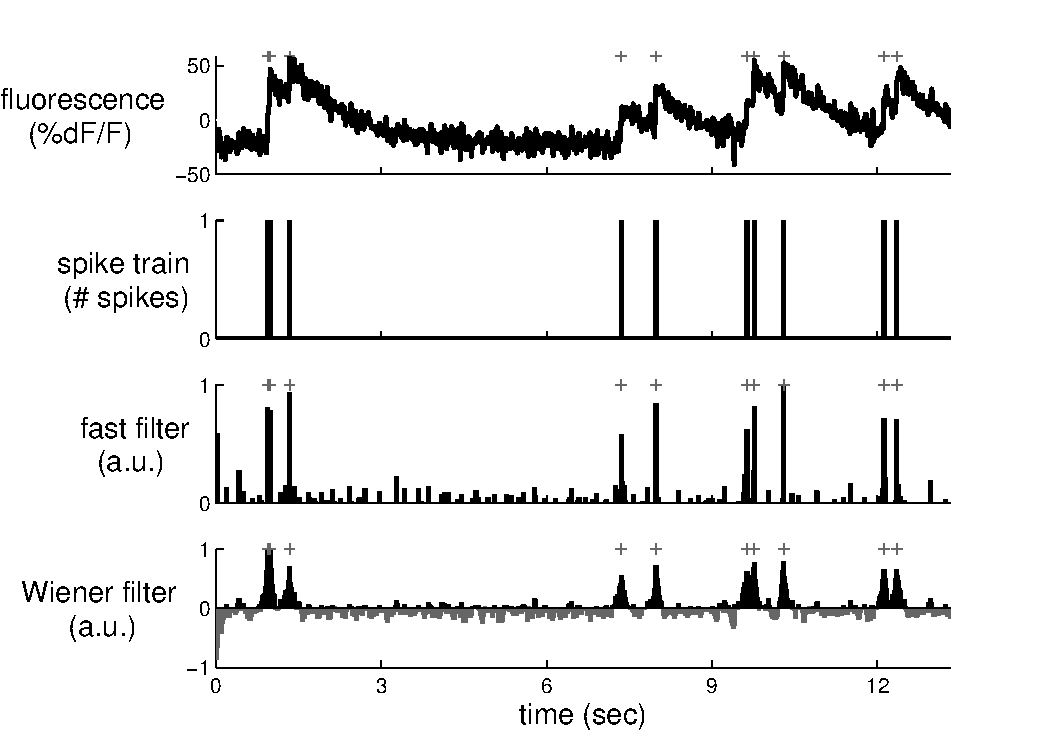
\includegraphics[width=.9\linewidth]{/Users/joshyv/Research/oopsi/fast-oopsi/figs/fast_wiener_inf13}
\caption[\foopsi filter outperforms Wiener filter]{A simulation showing that the \foopsi filter's inferred spike train is significantly more accurate than the output of the optimal linear deconvolution (Wiener filter). Note that neither filter constrains the inference to be a sequence of integers; rather, the \foopsi filter relaxes the constraint to allow all non-negative numbers, and the Wiener filter allows for all real numbers.  The restriction of the \foopsi filter to exclude negative numbers eliminates the ringing effect seen in the Wiener filter output, resulting in a much cleaner inference.  Note that the magnitude of the inferred spikes in the \foopsi filter output is proportional to the inferred calcium jump size.  Top panel: fluorescence trace.  Second panel: spike train.  Third panel: \foopsi filter inference.  Bottom panel: Wiener filter inference.  Note that the gray bars in the bottom panel indicate \emph{negative} spikes. Gray '$+$'s indicate true spike times.  Simulation details: $T= 400$ time steps, $\Del=33.3$ msec, $\alpha=1$, $\beta=0$, $\sig=0.2$, $\tau=1$ sec, $\lam=1$ Hz. Parameters and conventions are consistent across figures, unless indicated otherwise.} \label{fig:woopsi_inf}
\end{figure}

Figure \ref{fig:stats} quantifies the relative performance of the fast and Wiener filters.  The top left panel shows a typical simulated spike train (bottom),  a corresponding relatively low SNR fluorescence trace (middle), and a relatively high SNR fluorescence trace (top), as examples.  The top right panel compares the mean-squared-error (MSE) of the inferred spike trains using the fast (solid) and Wiener (dashed) filter, as a function of expected firing rate.  Clearly, the fast filter has a better (lower) MSE for all rates.  The bottom left panel shows a receiver-operator-characteristic (ROC) curve for another simulation.  Again, the fast filter dominates the the Wiener filter, have a higher true positive rate for every false negative rate.  Finally, the bottom right panel shows that the area-under-curve (AUC) of the fast filter is better (higher) than the Wiener filter until the noise is very large. Collectively, these analyses suggest that for a wide range of firing rates and signal quality, the fast filter outperforms the Wiener filter.  


\begin{figure}[h!]
\centering 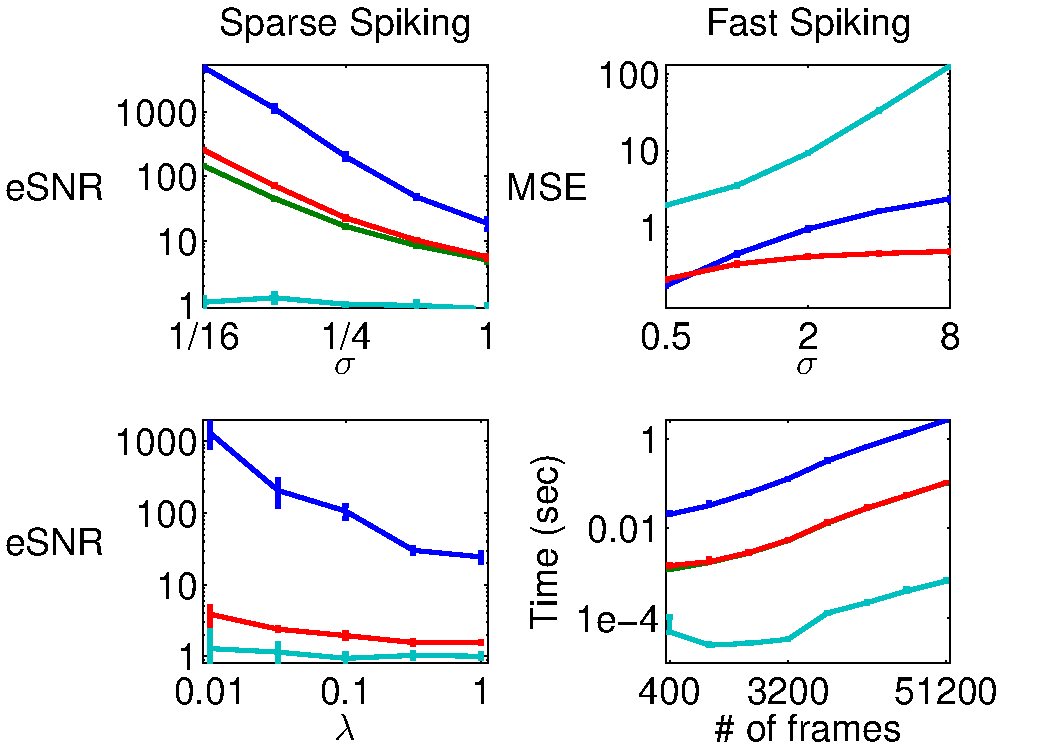
\includegraphics[width=.9\linewidth]{/Users/joshyv/Research/oopsi/fast-oopsi/figs/stats}
\caption[quantifying the relative accuracy for the fast and Wiener filters]{In simulations, the fast filter quantitatively and significantly achieves higher accuracy than the Wiener filter.  Top left panel: a spike train (bottom), and two simulated fluorescence traces, using the same spike train, one with low signal-to-noise-ratio (SNR) (middle), and one with high SNR (top).  Simulation parameters:  $\tau=0.5$ sec, $\lam=3$ Hz, $\Del=1/30$ sec, $\sig=0.6$ (low SNR) and $0.1$ (high SNR). Simulation parameters in other panels are the same, except where explicitly noted.  Top right panel: mean-squared-error (MSE) for the fast (solid line) and Wiener (dash-dotted line) filter, for varying the expected firing rate $\lambda$.  Note that both axes are on a log-scale.  Further note that the fast filter has a better (lower) MSE for all expected firing rates. Errorbars show standard deviation over 10 repeats. Simulation parameters: $\sig=0.2$, $T=1000$ time steps. Bottom left: Receiver-operator-characteristic (ROC) curve comparing the fast (solid line) and Wiener (dashed-dotted line) filter. Note that for any given threshold, the Wiener filter has a better (higher) ration of true positive rate to false positive rate. Simulation parameters as in top right panel, except $\sig=0.35$ and $T=10,000$ time steps.  Bottom right panel: Area-under-curve (AUC) for fast (solid line) and Wiener (dashed-dotted line) filter as a function of standard deviation $\sig$.  Note that the fast filter has a better (higher) AUC for all $\sig$ until noise gets very high.  The two simulated fluorescence traces in the top left panel show the bounds for standard deviation here.  Errorbars show standard deviation over 10 repeats.} \label{fig:stats}
\end{figure}

Although in Figure \ref{fig:woopsi_inf} the model parameters were provided, in the general case, the parameters are unknown, and must therefore be estimated from the observations (as described in section \ref{sec:learn}). Importantly, this algorithm does not require ``training'' data, i.e., there is no need for joint imaging and electrophyiological experiments to estimate the parameters governing the relationship between the two.  Figure \ref{fig:woopsi_learn} shows another simulated example; in this example, however, the parameters are estimated from the observed fluorescence trace alone.  Again, it is clear that the \foopsi filter far outperforms the Wiener filter.

\begin{figure}[h!]
\centering 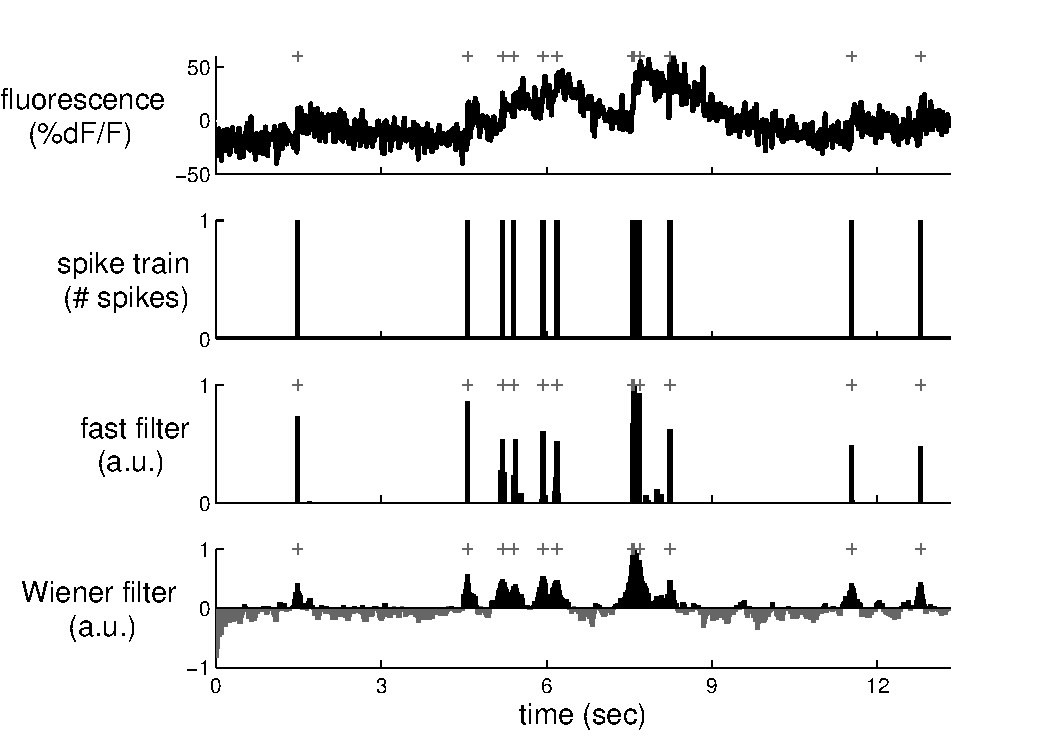
\includegraphics[width=.9\linewidth]{/Users/joshyv/Research/oopsi/fast-oopsi/figs/fast_wiener_learn13}
\caption[parameters may be estimated using the \foopsi filter]{A simulation showing that the \foopsi filter achieves significantly more accurate inference than the Wiener filter, even when the parameters unknown.  For both filters, the appropriate parameters were estimated using only the data shown above, unlike Figure \ref{fig:woopsi_inf}, in which the true parameters were provided to the filters. Simulation details different from those in Figure \ref{fig:woopsi_inf}: $T=1000$ time steps, $\Del=16.7$ msec, $\sig=0,4$.} \label{fig:woopsi_learn}
\end{figure}

Given the above two results, the \foopsi filter was applied to real data.  More specifically, by jointly recording electrophysiologically and imaging, the true spike times are known, and the accuracy of the two filters can be compared.  Figure \ref{fig:woopsi_data} shows a result typical of the 12 joint electrophysiological and imaging experiments conducted. As in the simulated data, the fast filter output is much ``cleaner'' than the Wiener filter, spikes are more well defined, and not spread out, due to the sparse prior imposed by the exponential approximation, as opposed to the smoothness prior imposed by the Wiener filter.  Note that the SNR of this trace is quite poor, which results in some false positives in the fast filter.  Regardless, the fast filter output is still more accurate than the Wiener filter, both as determined qualitatively by eye, and as quantified (described below).  Furthermore, although it is difficult to see in this figure, the first four ``events'' are actually pairs of spikes, which is reflected by the width and height of the corresponding inferred spikes when using the \foopsi filter. %(see Figure \ref{fig:woopsi_data_doublets} for a temporally zoomed in version from similar data). 
This suggests that although the scale of $\mb{n}$ is arbitrary, the \foopsi filter can correctly ascertain the number of spikes within spike events.  

\begin{figure}[h!]
\centering 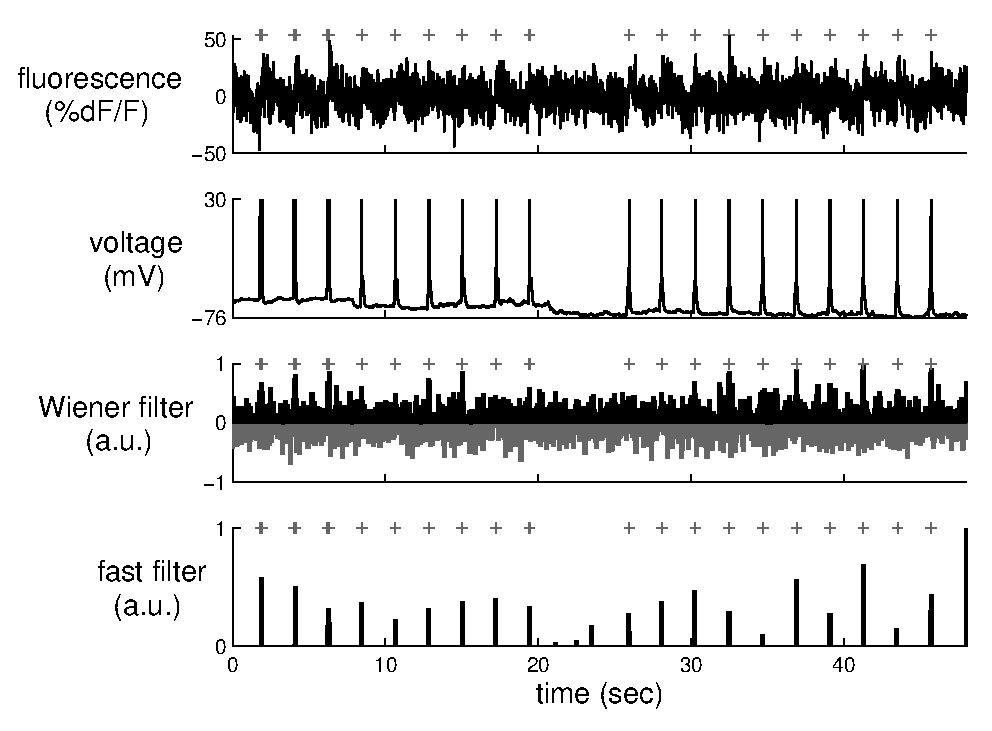
\includegraphics[width=.9\linewidth]{/Users/joshyv/Research/oopsi/fast-oopsi/figs/fast_wiener_vitro4}
\caption[\foopsi filter outperforms Wiener filter on biological data]{Typical in vitro data showing that the \foopsi filter significantly outperforms the Wiener filter, using OGB-1. Note that all the parameters for both filters were estimated only from the fluorescence data in the top panel (ie, not considering the voltage data at all).  '$+$'s denote true spike times extracted from the patch data, not inferred spike times from $\mb{F}$.} \label{fig:woopsi_data}
\end{figure}


Figure \ref{fig:woopsi_data_doublets} further evaluates this claim.  While recording and imaging, the cell was forced to spike once, twice, or thrice, for each spiking event.  Na\"{i}vely, this would suggest that an algorithm based on a purely linear model would struggle to resolve spike fidelity in this high frequency spiking regime.  However, the \foopsi filter infers the correct number of spikes in each event.  On the contrary, there is no obvious way to count the number of spikes within each event when using the Wiener filter. We confirm this impression by computing the correlation coefficient, $r^2$ between the sum of each filter's output and the true number of spikes, for all 12 joint electrophysiological and imaging traces.  Indeed, while the fast filter's $r^2$ was $0.47$, the Wiener filter's $r^2$ was $-0.01$ (after thresholding all negative spikes), confirming that the Wiener filter output can not reliably convey the number of spikes in a fluorescence trace, whereas the fast filter can.  Furthermore, varying the magnitude of the threshold for the Wiener filter to discard more ``low-amplitude noise'' could increase the magnitude of $r^2$, up to $0.24$, still significantly lower than the fast filter's $r^2$ value.  On the other hand, no amount of thresholding the fast filter yielded an improved $r^2$, indicating that thresholding the output of the fast filter is unlikely to improve spike inference quality.

\begin{figure}[h!]
\centering 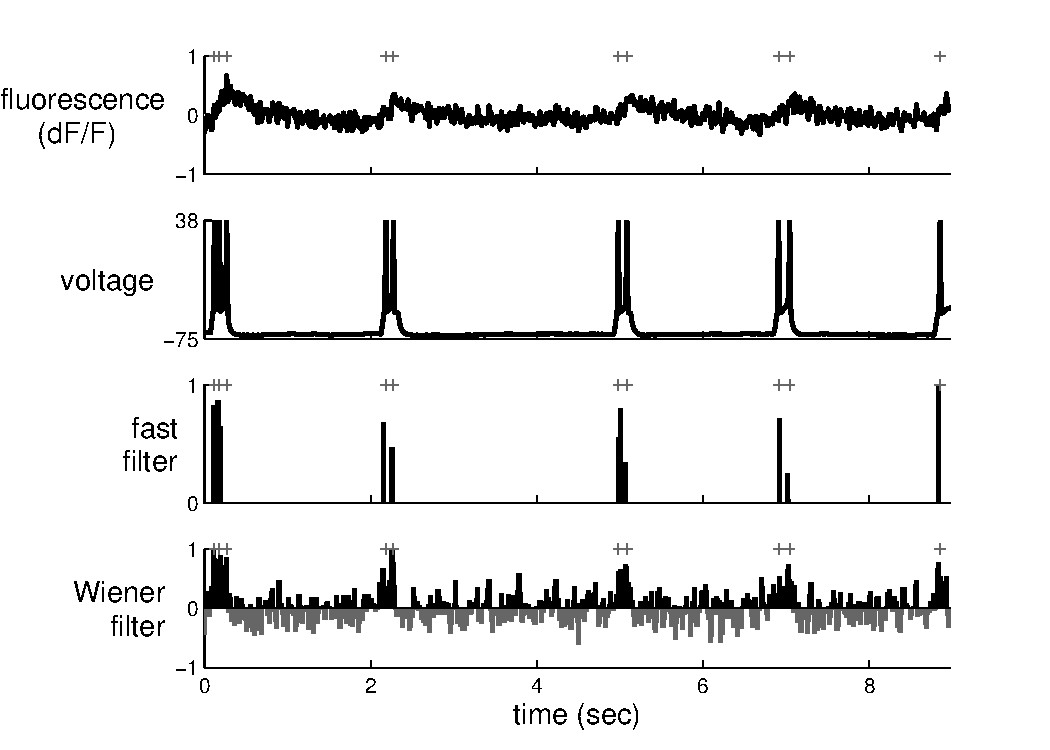
\includegraphics[width=.9\linewidth]{/Users/joshyv/Research/oopsi/fast-oopsi/figs/fast_wiener_burst12}
\caption[\foopsi filter outperforms Wiener filter on multi-spike events]{Typical in vitro data with multi-spike events, showing that the \foopsi filter can often resolve the correct number of spikes within each spiking event, while imaging using OGB-1, given sufficiently high SNR.  It is difficult, if not impossible, to count the number of spikes given the Wiener filter output.  Recording and fitting parameters as in Figure \ref{fig:woopsi_data}. Note that the parameters were estimated using a 60 sec long recording, of which only a fraction is shown here, to more clearly depict the number of spikes per event.  } \label{fig:woopsi_data_doublets}
\end{figure}




% \begin{figure}[h!]
% \centering 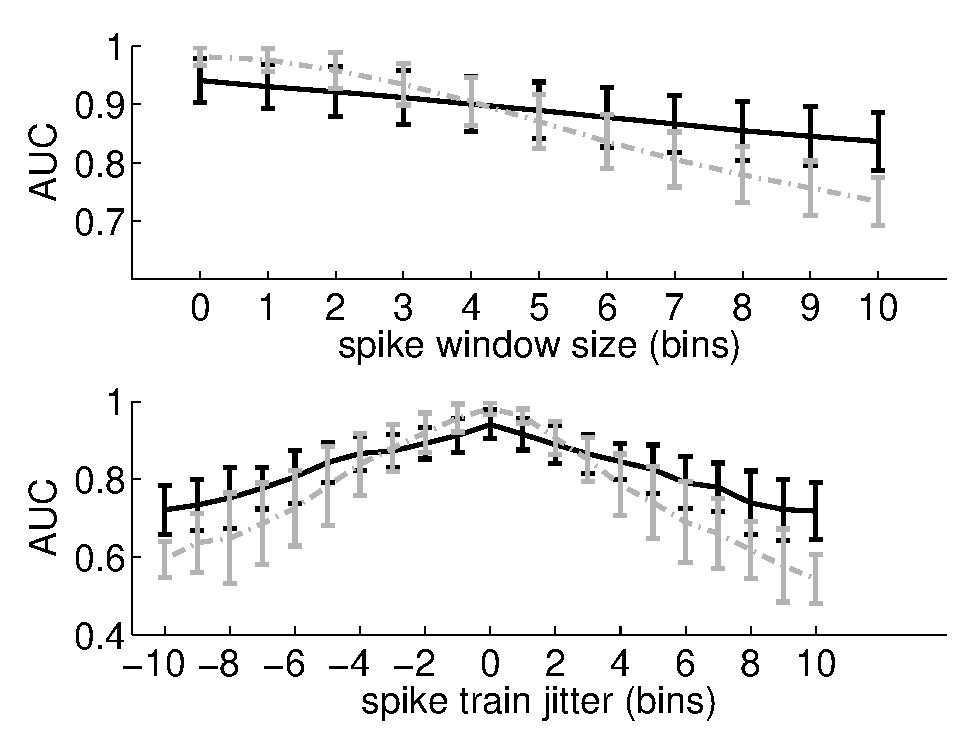
\includegraphics[width=.9\linewidth]{/Users/joshyv/Research/oopsi/fast-oopsi/figs/stats_data}
% \caption{Quantitative comparison---using in vitro data---of fast (black line) and Wiener (gray line) filter performance.  For each data set with both electrophysiology and imaging data, we can compute the generalized area-under-curve (gAUC), which counts positives as true within a given window size.  gAUC was computed for each cell, mean (line) and standard deviation (errorbars) are show in the two panels.  In the top panel, windows are symmetric, meaning allow inferred spike to be off by $\pm k$ bins, where $k=0,\ldots, 10$.  In the bottom panel, windows are asymmetric.  Note the lack of systematic bias, and that with small window sizes, both algorithms perform similarly, but with larger bin windows, the fast filter is significantly more accurate than the Wiener filter. } \label{fig:stats-data}
% \end{figure}





\subsection{Online analysis of spike trains using the \foopsi filter}

A central aim for this work was the development of an algorithm that infers spikes fast enough to use online while imaging a large population of neurons (eg, $> 100$).  Figure \ref{fig:pop} shows a segment of the results of running the \foopsi filter on 136 neurons, recorded simultaneously, as described in section \ref{sec:exp}.  Note that the filtered fluorescence signals show fluctuations in spiking much more clearly than the unfiltered fluorescence trace. These spike trains were inferred in less than imaging time, meaning that one could infer spike trains for the past experiment while conducting the subsequent experiment. More specifically, a movie with 5,000 frames of 100 neurons can be analyzed in about ten seconds on a standard desktop computer.  Thus, if that movie was recorded at 50 Hz, while collecting the data required 100 seconds, inferring spikes only required ten seconds, a ten-fold improvement over real-time.  


\begin{figure}[h!]
\begin{centering} 
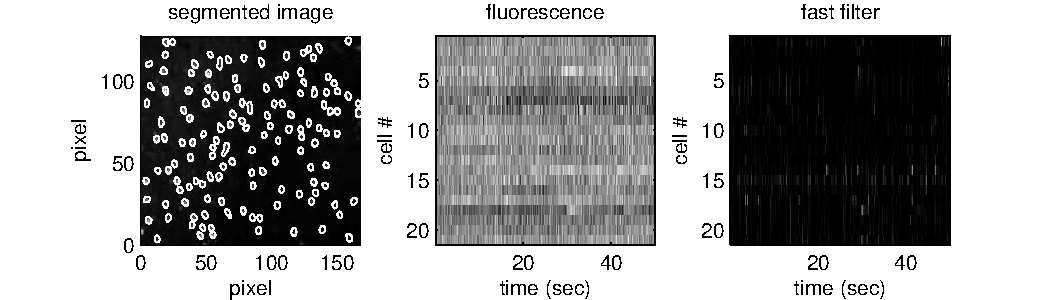
\includegraphics[width=1\linewidth]{/Users/joshyv/Research/oopsi/fast-oopsi/figs/pop}
\end{centering}
\caption[\foopsi filter is robust and works online for populations of neurons]{The \foopsi filter infers spike trains from a large population of neurons imaged simultaneously \emph{in vitro}, using Fura-2, faster than real-time.  Specifically, inferring the spike trains from this 400 sec long movie including 136 neurons required only about 40 sec on a standard laptop computer. The inferred spike trains much more clearly convey neural activity than the raw fluorescence traces.  Although no intracellular ``ground truth'' is available on this population data, the noise seems to be reduced, consistent with the other examples with ground truth.  Left panel: Mean image field, automatically segmented into ROIs each containing a single neuron using custom software.  Middle panel: example fluorescence traces.  Right panel: \foopsi filter output corresponding to each associated trace. Note that neuron identity is indicated by color across the three panels.} \label{fig:pop}
\end{figure}


\subsection{Extensions}

Section \ref{sec:model} describes a simple principled first-order model relating the spike trains to the fluorescence trace. A number of the simplifying assumptions can be straightforwardly relaxed, as described below.


\subsubsection{Replacing Gaussian observations with Poisson}

In the above, observations were assumed to have a Gaussian distribution.  The statistics of photon emission and counting, however, suggest that a Poisson distribution would be more natural, especially for two-photon data \cite{SjulsonMiesenbock07}, yielding:
\begin{align} \label{eq:poiss}
	F_t \overset{iid}{\sim}\text{Poisson}(\alpha C_t + \beta).
\end{align}
One additional advantage to this model over the Gaussian model, is that the variance parameter, $\sig^2$, no longer exists, which might make learning the parameters simpler.  Importantly, the log-posterior is still concave in $\mb{C}$, as
the prior remains unchanged, and the new log-likelihood term is a sum of terms concave in $\mb{C}$:
\begin{align}
	\log P[\mb{F} | \mb{C}] = \sum_{t=1}^T \log P[F_t | C_t ] = \sum_{t=1}^T \{F_t \log (\alpha C_t + \beta) -(\alpha C_t + \beta) - \log(F_t !)\}.
\end{align}
The gradient and Hessian of the log-posterior can therefore be computed analytically by substituting the above likelihood terms for those implied by Eq.~\eqref{eq:F}.  In practice, however, modifying the filter for this model extension did not seem to significantly improve inference results in any simulations or data (not shown).

\subsubsection{Allowing for a time-varying prior}

In Eq.~\eqref{eq:n}, the rate of spiking is a constant.  Often, additional knowledge about the experiment, including external stimuli, or other neurons spiking, can provide strong time-varying prior information \cite{VogelsteinPaninski09}.  A simple model modification can incorporate that feature:
\begin{align}
	n_t &\overset{iid}{\sim} \text{Poisson}(\lam_t \Del),
\end{align}
where $\lam_t$ is now a function of time.  Approximating this time-varying Poisson with a time-varying exponential with the same time-varying mean (similar to Eq.~\eqref{eq:obj2}), and letting $\mb{\lam} = [\lam_1, \ldots, \lam_T]\T \Del$, yields an objective function identical to Eq.~\eqref{eq:eta3}, so log-concavity is maintained, and the same techniques may be applied.  However, as above, this model extension did not yield any significantly improved filtering results (not shown).

\subsubsection{Saturating fluorescence}

Although all the above models assumed a \emph{linear} relationship between $F_t$ and $C_t$, the relationship between fluorescence and calcium is typically better approximated by the nonlinear Hill equation \cite{PologrutoSvoboda04}. Modifying Eq.~\eqref{eq:F} to reflect this change yields: 
\begin{align}
	F_t &= \alpha \frac{C_t}{C_t+k_d} + \beta +  \sig \varepsilon_t, \qquad \varepsilon_t \overset{iid}{\sim} \mc{N}(0,1).
\end{align}
Importantly, log-concavity of the posterior is no longer guaranteed in this nonlinear model, meaning that converging to the global maximum is no longer guaranteed.  Assuming a good initialization can be found, however, if this model is more accurate, then ascending the gradient for this model might yield improved inference results.  In practice, initializing with the  inference from the \foopsi filter assuming a linear model (eg, Eq.~\eqref{eq:overlapping}) often resulted in nearly equally accurate inference, but inference assuming the above nonlinearity was far less robust than the inference assuming the linear model (not shown).  
%Unfortunately, using this more powerful model did not result in substantial inference improvements for simulated or \emph{in vitro} data (not shown).  This is possibly due to approximating the Poisson distribution governing spiking with an exponential distribution.  This approximation is required to ensure concavity of the posterior.  

\subsubsection{Using the \foopsi filter to initialize the sequential Monte Carlo filter}

A sequential Monte Carlo (SMC) method to infer spike trains can incorporate this saturating nonlinearity, as well as the other model extensions discussed above \cite{VogelsteinPaninski09} . However, this SMC filter is not nearly as computationally efficient as the fast filter proposed here.  Like the \foopsi filter, the SMC filter estimates the model parameters in a completely unsupervised fashion, i.e.,  from the fluorescence observations, using an expectation-maximization algorithm (which requires iterating between computing the expected value of the hidden variables --- $\mb{C}$ and $\mb{n}$ --- and updating the paramters).  In \cite{VogelsteinPaninski09}, parameters for the SMC filter were initialized based on other data.  While effective, this initialization was often far from the final estimates, and therefore, required a relatively large number of iterations (eg, 20--25) before converging.  Thus, it seemed that the \foopsi filter could be used to obtain an improvement to the initial parameter estimates, given an appropriate rescaling to account for the nonlinearity, thereby reducing the required number of iterations to convergence.  Indeed, Figure \ref{fig:smc_init} shows how the SMC filter outperforms the \foopsi filter on biological data, and only required 3--5 iterations to converge on this data, given the initialization from the \foopsi filter (which was typical).  Note that the first few events of the spike train are individual spikes, resulting in relatively small fluorescence fluctuations, whereas the next events are actually spike doublets or triplets, causing a much larger fluorescence fluctuation.  Only the SMC filter picks up the individual spikes in this trace, a result typical when the effective SNR is poor.  Thus, these two inference algorithms are complementary: the \foopsi filter can be used for rapid, online inference, and for initializing the SMC filter, which can then be used to further refine the spike train estimate.  Importantly, although the SMC filter often outperforms the \foopsi filter, the \foopsi filter is more robust, meaning that it more often works ``out-of-the-box.''

\begin{figure}[h!]
\centering 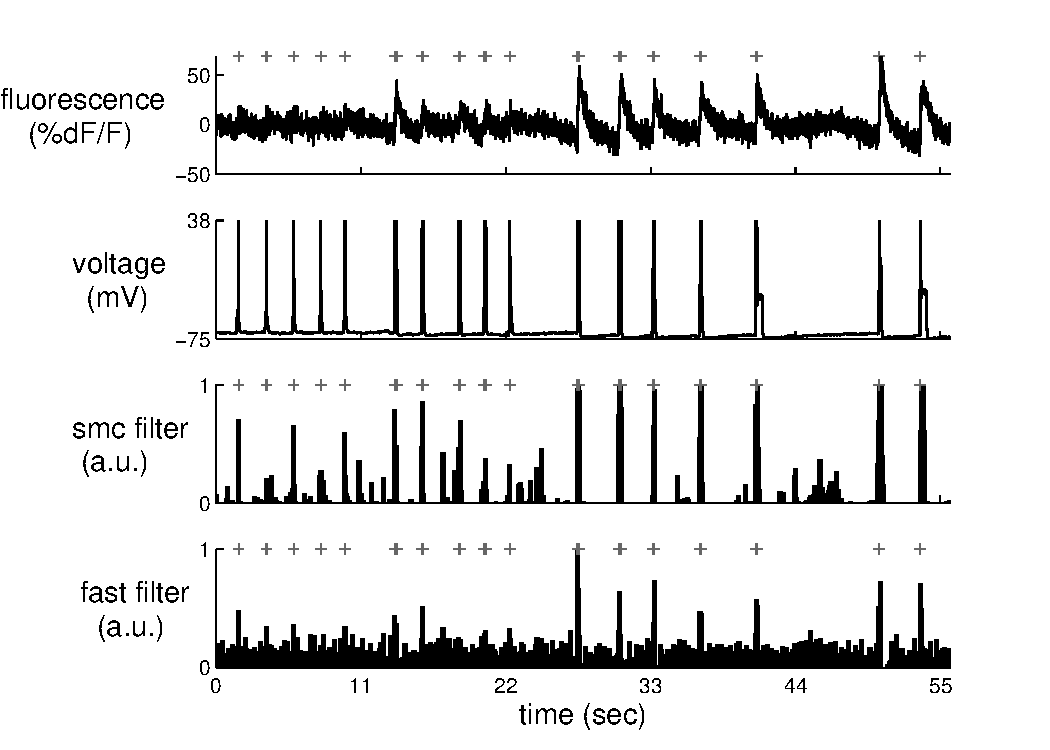
\includegraphics[width=.9\linewidth]{/Users/joshyv/Research/oopsi/fast-oopsi/figs/fast_smc_vitro12}
\caption[\foopsi filter can initialize Wiener filter]{in vitro data with poor SNR depicting the \foopsi filter effectively initializing the parameters for the SMC filter, significantly reducing the number of expectation-maximization iterations to convergence, using OGB-1.  Note that while the \foopsi filter clearly infers the spiking events in the end of the trace, those in the beginning of the trace are less clear.  On the other hand, the SMC filter more clearly separates non-spiking activity from true spikes.  Also note that the ordinate on the bottom panel corresponds to the inferred probability of a spike having occurred in each frame.} \label{fig:smc_init}
\end{figure}

\subsection{Spatial filter} \label{sec:results:spatial}

In the above, the filters operated on one-dimensional fluorescence traces. Typically, the data are time-series of images which are first segmented into regions-of-interest (ROI), and then (usually) spatially averaged to obtain a one-dimensional time-series, $\mb{F}$.  In theory, one could improve the effective SNR of the fluorescence trace by scaling each pixel according to their SNR.  In particular, pixels not containing any information about calcium fluctuations can be ignored, and pixels that are partially anti-correlated with one another could have weights with opposing signs.  

Figure \ref{fig:spatial} demonstrates the potential utility of this approach.  The top row shows different depictions of an ROI containing a single neuron.  On the far left panel is the true spatial filter for this neuron.  This particular spatial filter was chosen based on experience analyzing both \emph{in vitro} and \emph{in vivo} movies; often, it seems that the pixels immediately around the soma are anti-correlated with those in the soma.  This effect is possibly due to the influx of calcium from the extracellular space immediately around the soma.   The standard approach, given such a noisy movie, would be to first segment the movie to find an ROI corresponding to the soma of this cell, and then spatially average all the pixels found to be within this ROI.  The second panel shows this standard ``boxcar spatial filter.''  The third panel shows the mean frame. The fourth panel shows the learned filter, using Eq.~\eqref{eq:alpha_x2} to estimate the spatial filter and background. Clearly, the learned filter is very similar to the mean filter and the true filter. 

The bottom panels of Figure \ref{fig:spatial} depict the effect of using the various spatial filters. The middle panels show the fluorescence trace (black line) and true spike train (gray $+$'s).  The bottom panels show the infer spike trains (black bars) using these various spatial filters, and again the true spike train (gray $+$'s).  While the performance is very similar for all of them, the boxcar filter's inferred spike train is not as clean.  




\begin{figure}[h!]
\centering 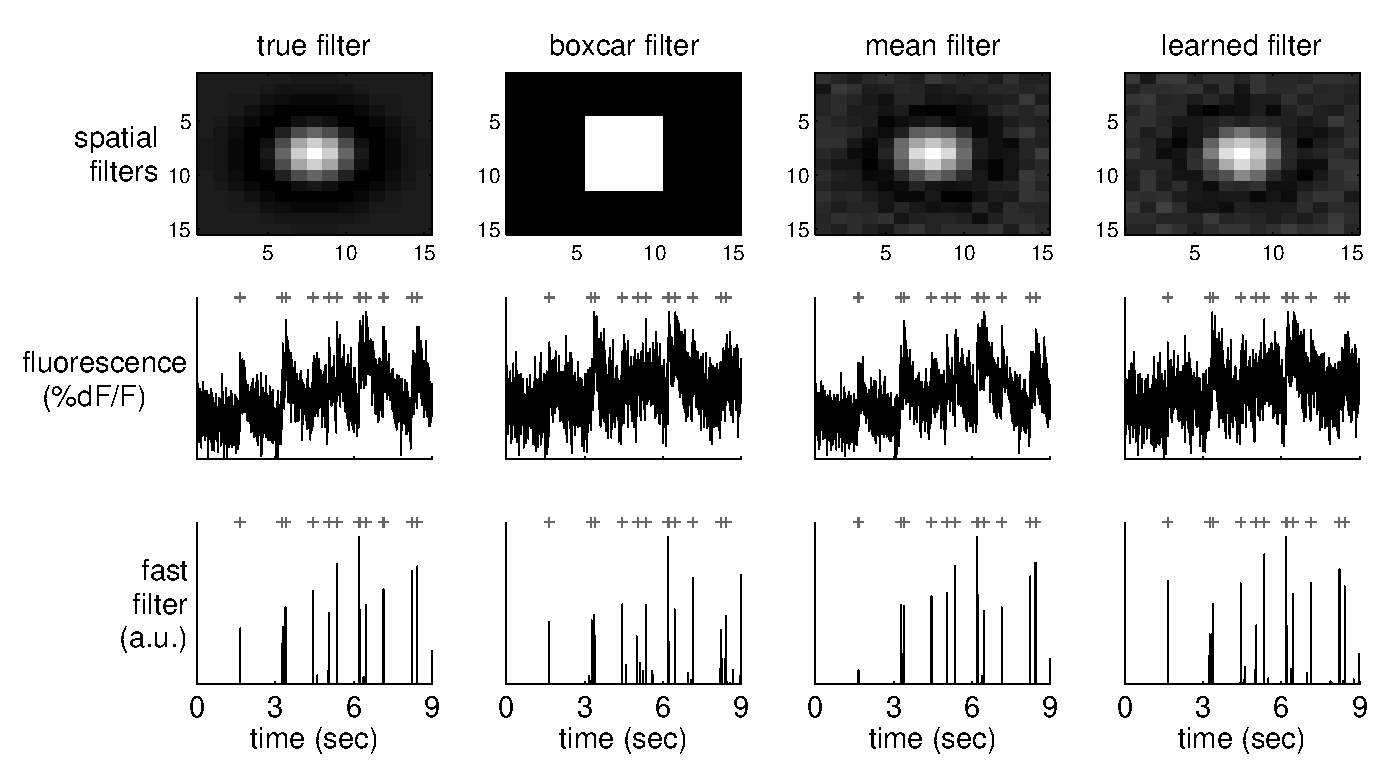
\includegraphics[width=.9\linewidth]{/Users/joshyv/Research/oopsi/fast-oopsi/figs/spatial_inf}
\caption[spatial filtering can improve effective SNR]{A simulation demonstrating that using a better spatial filter can significantly enhance the effective SNR. The true spatial filter was a difference of Gaussians: a positively weighted Gaussian of small width, and a negatively weighted Gaussian with larger width (both with the same center).  Each column shows the spatial filter (top), one-dimensional fluorescence projection using that spatial filter (middle), and inferred spike train (bottom).  From left to right, columns use the true, boxcar, mean, and learned spatial filter, obtained using Eq.~\eqref{eq:alpha_x2}. Simulation parameters: $\mv{\alpha}=\mc{N}(\ve{0},2 \mb{I})-0.5 \mc{N}(\ve{0},2.5 \mb{I})$ where $\mc{N}(\ve{\mu},\ve{\Sig})$ indicates a two-dimensional Gaussian with mean $\ve{\mu}$ and covariance matrix $\ve{\Sig}$, $\mv{\beta}=\ve{0}$, $\sig=0.2$, $\tau=0.85$ sec, $\lam=5$ Hz, $\Del=5$ msec, $T=1200$ time steps.} \label{fig:spatial} 
\end{figure}



\subsection{Overlapping spatial filters} \label{sec:results:overlapping}


The above shows that if a ROI contains only a single neuron, the effective SNR can be enhanced by spatially filtering.  However, this analysis assumes that only a single neuron is in the ROI.  Often, ROIs are overlapping, or nearly overlapping, making the segmentation problem more difficult.  Therefore, it is desirable to have an ability to crudely segment, yielding only a few neurons in each ROI, and then spatially filter within each ROI to pick out the spike trains from each neuron.  This may be achieved in a principled manner by generalizing the model as described in section \ref{sec:methods:overlapping}.  %Figure \ref{fig:spatial_multi_inf} shows how this approach can separate the two signals, assuming that the spatial filters of the two neurons are known.  %Note that the spatial filters are sufficiently overlapping that some ``bleed-though'' can be seen across the traces.  
%While Figure \ref{fig:spatial_multi_inf} shows that one could separate the signals if the spatial filters of the neurons were known, 
Typically, the true spatial filters of the neurons in the ROI will be unknown, and thus, must be estimated from the data.  This problem may be considered a special case of blind source separation \cite{BellSejnowski95, MukamelSchnitzer09}. Figure \ref{fig:spatial_multi_learn} shows that multiple signals can be separated, with reasonable assumptions on correlations between the signals, and SNR.  Note that separation occurs even though the signal is significantly overlapping (top panels). To estimate the spatial filters, they are initialized using the boxcar filters (middle panels).  After a few iterations, the spatial filters converge to very close approximation to the true spatial filters (compare true (left) and learned (right) spatial filters for the two neurons).  Note that both the true and learned spatial filters yield much improved spike inference relative to the boxcar filter.  This suggests that even when multiple neuron's spatial filters are significantly overlapping, each spike train is potentially independently recoverable.  




% \begin{figure}[h!]
% \centering \includegraphics[width=.9\linewidth]{/Users/joshyv/Research/oopsi/fast-oopsi/figs/spatial_inf_multi}
% \caption[overlapping spatial filters are not problematic]{Simulation showing that even when two neurons' spatial filters are overlapping, one can separate the two spike trains by spatial filtering. Top left panel: mean frame from the movie.  Bottom left: optimal one-dimensional fluorescence projections for the neuron 1 (black line) and neuron 2 (gray line), and their respective spike trains (black and gray '$+$' symbols, respectively).  Top middle panel: the true spatial filter for neuron 1.  Bottom middle panel: inferred (black line) and true (black '$+$' symbols) spike trains.  Top right panel: the true spatial filter for neuron 2.   Bottom right panel: inferred (gray line) and true (gray '$+$' symbols) spike trains. Simulation details: $\mv{\alpha}^1=\mc{N}([-1.8, 1.8]\T,2 \mb{I})\, \mv{\alpha}^2=\mc{N}([1.8, -1.8]\T,5 \mb{I})$, $\mv{\beta}=\ve{0}$, $\tau=[0.5, 0.5]\T$ sec, $\lam=[1.5, 1.5]\T$ Hz.} \label{fig:spatial_multi_inf}
% \end{figure}



\begin{figure}[h!]
\centering 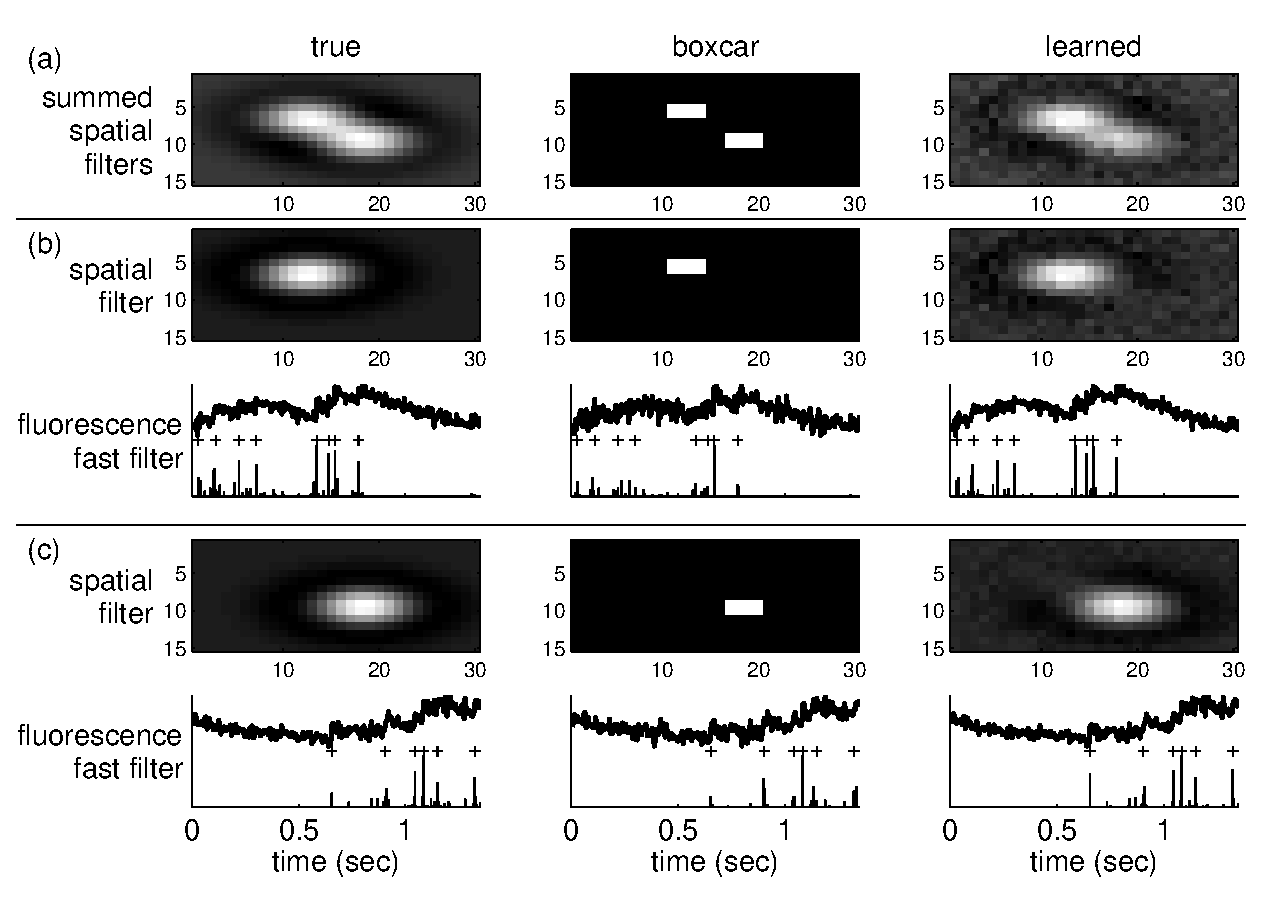
\includegraphics[width=.9\linewidth]{/Users/joshyv/Research/oopsi/fast-oopsi/figs/spatial_learn_multi}
\caption[overlapping spatial filters can be estimated]{Simulation showing that when two neurons' spatial filters are largely overlapping, learning the optimal spatial filters using Eq.~\ref{eq:alpha_x3} can yield improved inference of the typical boxcar type filters.  Simulation parameters: $\mv{\alpha}^1=\mc{N}([-1, 0],2 \mb{I})-0.5 \mc{N}([-1, 0],2.5 \mb{I})$, $\mv{\alpha}^2=\mc{N}([1, 0],2 \mb{I})-0.5 \mc{N}([1, 0],2.5 \mb{I})$, $\mv{\beta}=\ve{0}$,  $\sig=0.02$, $\tau=0.5$ sec, $\lam=5$ Hz, $\Del=5$ msec, $T=1200$ time steps (not all time steps are shown).} \label{fig:spatial_multi_learn}
\end{figure}



% \begin{figure}[h!]
% \centering 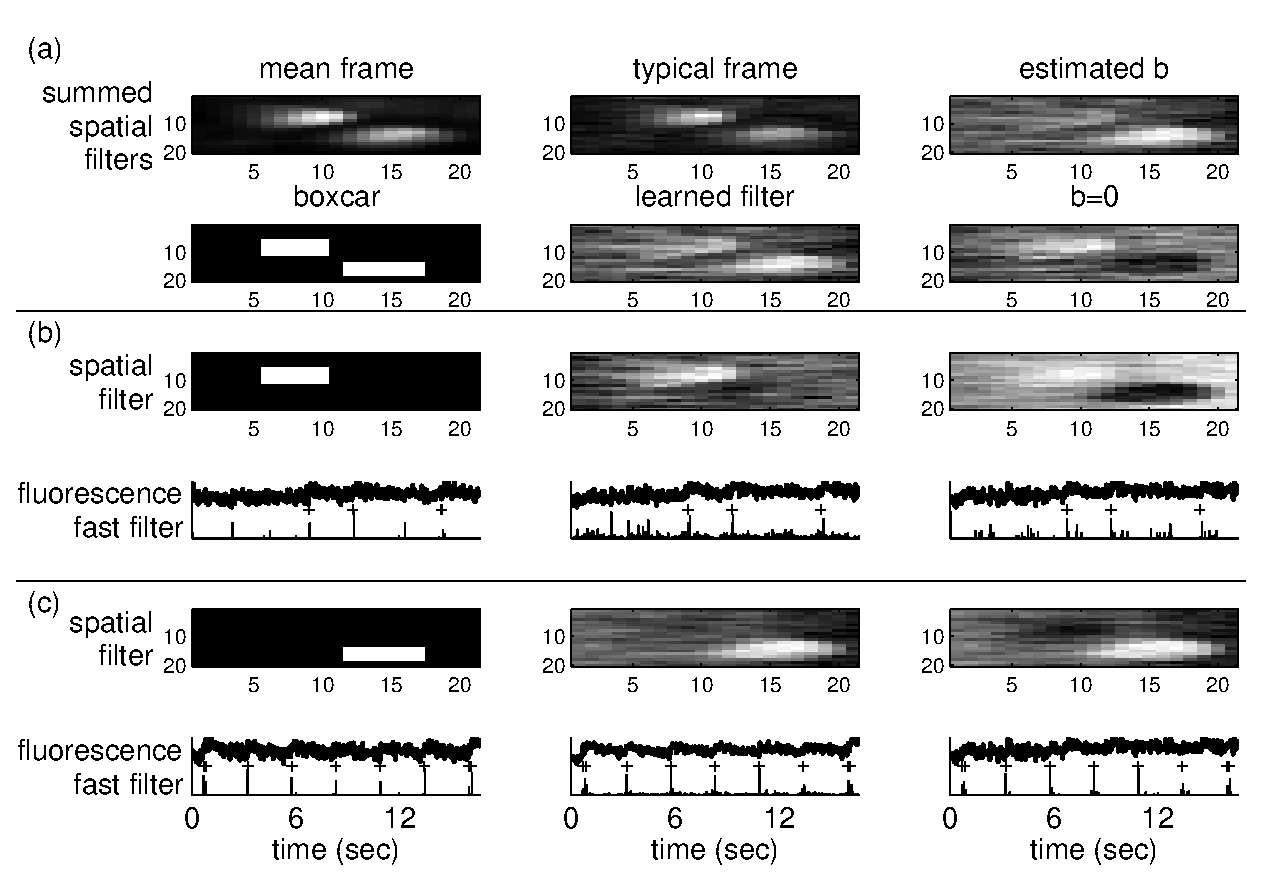
\includegraphics[width=.9\linewidth]{/Users/joshyv/Research/oopsi/fast-oopsi/figs/spatial_learn_multi_vitro}
% \caption[overlapping spatial filters can be estimated]{in vitro spatial filtering improves inference results.} \label{fig:spatial_multi_learn}
% \end{figure}





\section{Discussion} \label{sec:dis}

% \paragraph{Summary}


This work describes an algorithm that finds the approximate \emph{maximum a posteriori} (MAP) spike train, given a calcium fluorescence movie.  The approximation is required because finding the actual MAP estimate is not currently computationally tractable.  Replacing the assumed Poisson distribution on spikes with an exponential distribution yields a log-concave optimization problem, which can be solved using standard gradient ascent techniques (such as Newton-Raphson).  This exponential distribution has an advantage over a Gaussian distribution by restricting spikes to be positive, which improves inference quality (cf. Figure \ref{fig:woopsi_inf}), is a better approximation to a Poisson distribution with low rate, and imposes a sparse constraint on spiking. Furthermore,  all the parameters can be estimated from only the fluorescence observations, obviating the need for joint electrophysiology and imaging (cf. Figure \ref{fig:woopsi_learn}).  This approach is robust, in that it works ``out-of-the-box'' on all the \emph{in vitro}  data analyzed (cf. Figure \ref{fig:woopsi_data} and Figure \ref{fig:woopsi_data_doublets}). By utilizing the special banded structure of the Hessian matrix of the log-posterior, this approximate MAP spike train can be inferred fast enough on standard computers to use it for online analyses of over 100 neurons simultaneously (cf. Figure \ref{fig:pop}).


Finally, the \foopsi filter is based on a biophysical model capturing key features of the data, and may therefore be straightforwardly generalized in several ways to improve accuracy.  Unfortunately, some of these generalizations do not improve inference accuracy, perhaps because of the exponential approximation.  Instead, the \foopsi filter output can be used to initialize the more general SMC filter \cite{VogelsteinPaninski09}, to further improve inference quality (cf. Figure \ref{fig:smc_init}).  Another model generalization allows incorporation of spatial filtering of the raw movie into this approach (cf. Figure \ref{fig:spatial}). Even when multiple neurons are overlapping, spatial filters may be estimated to obtain improved spike inference results (cf. Figure \ref{fig:spatial_multi_learn}).

Ideally, one could compute the full joint posterior of entire spike trains, conditioned on the fluorescence data.  This distribution is analytically intractable, due to the Poisson assumption on spike trains.  A Bayesian approach could use Markov Chain Monte Carlo methods to recursively sample spikes until a whole sample spike train is obtained \cite{AndrieuDoucet01,MishchenkoPaninski09,JouclaPouzat10}.  Because a central aim here was computational expediency, two alternatives to fully Bayesian strategy are natural: approximating the posterior, or using a ``greedy'' approach. A ``greedy'' approach is natural: i.e.,  recursively sample the most likely spike, update the posterior, and repeat until the posterior stops increasing.  Template matching, projection pursuit regression \cite{FS81}, and matching pursuit \cite{MallatZhang93} are examples of such a greedy approach (Greenberg et al's algorithm \cite{GreenbergKerr08} could also be considered a special case of such a greedy approach).  Both the greedy methods, and the one developed here, aim to optimize a similar objective function.  While greedy methods reduce the computational burden by restricting the search space of spike trains, this approach utilized analytic approximations.  The advantage of the greedy approaches relative to this one is that greedy approaches result in spike trains (ie, a binary sequence).  However, because of the numerical approximations and restrictions, one can never be sure whether the algorithm finds the \emph{most} likely possible spike train.  On the other hand, the approach developed herein is guaranteed to quickly find the most likely spike ``train'', but now the inferred spike train allows for partial spikes.  

A number of additional extensions follow from this work.  First, pairing this filter with a crude but automatic segmentation tool to obtain ROIs would create a completely automatic algorithm that converts raw movies of populations of neurons into populations of spike trains.  Second, this filter could be coupled with more sophisticated algorithms to initialize the spatial filters when they are overlapping  \cite{MukamelSchnitzer09}. Furthermore, one could regularize the inferred spatial filters, using an elastic net type approach \cite{ZouHastie05,GrosenickSmith09}.


Third, while the Poisson distribution was approximated with an exponential distribution here, other analytic approximations are possible. For instance, the Gaussian approximation is more appropriate for high firing rates, although in simulations, this more accurate approximation did not improve the Wiener filter output relative to the fast filter output (cf. Figure \ref{fig:stats}).  Another approach would be to approximate the $\log (n!)$  term from the exponential distribution (which makes the log-likelihood non-concave) using Stirling's formula. However, this approximation is only accurate for $n\gg 1$ \cite{AbramowitzStegun64}, and is therefore inappropriate in this low firing rate regime.  Perhaps the best approximation one could implement would be to compute the closest log-concave relaxation to the Poisson model \cite{KoenkerMizera10}. More formally, let $P(i)$ represent the Poisson mass at $i$, and let $\log Q$ be some concave density.  Then, one could find the log-density $Q$ such that $Q$ maximizes $\sum_i P(i) Q(i) - \int \exp[Q(x)] dx$ over the space of all concave $Q$. The first term corresponds to the log-likelihood, equivalent to the Kullback–Leibler divergence \cite{CoverThomas91}, and the second is a Lagrange multiplier to ensure that the density $\exp(Q)$ integrates to unity. This is a convex problem because the space of all concave $Q$ is convex, and the objective function is concave in $Q$. In addition, it is easy to show that the optimal $Q$ has to be piecewise linear; this means that one need not search over all possible densities, but rather, simply vary $Q(i)$ at the integers. Note that $\int \exp[Q(x)] dx$ can be computed explicitly for any piecewise linear $Q$. This optimization problem can be solved using simple interior point methods, and in fact the Hessian of the inner loop of the interior point method will be banded (because enforcing concavity of $Q$ is a local constraint). This approximation could potentially be more accurate than our exponential approximation, and is therefore of interest for future work. Regardless of how the analytic approximation is made, one could imagine initializing a greedy approach using the output of an analytic approximation approach to combine the power of the two.  

Fourth, in this work, we made two simplifying assumptions that can easily be relaxed: (i) instantaneous rise time of the fluorescence transient after a spike, and (ii) constant background.  In practice, often either or both of these assumptions are inaccurate.  Specifically, genetic sensors tend to have a much slower rise time than organic dyes \cite{ReiffBorst05}.  Further, the background often exhibits slow baseline drift due to movement, temperature fluctuations, laser power, etc., not to mention bleaching, which is ubiquitous for long imaging experiments.  Both slow rise and baseline drift can be incorporated into our forward model using the following generalization. Let $\mb{X}=(X_1, \ldots, X_n)$, where $n$ is the dimensionality of the signal, be a multidimensional time varying signal.  Different elements of $\mb{X}$ might correspond to different calcium extrusion mechanisms with different time constants, or different sources of baseline drift.  Further let $\Gam$ be a $n \times n$ matrix, and $\mb{A}$ and $\mb{a}$ be $n \times 1$ element vector.  Then, we have:
\begin{align}
	F_t &= \mb{\alpha}\T \mb{X}_t + \beta + \eps, \qquad& \eps \overset{iid}{\sim} \mc{N}(0,1) \\
	\mb{X}_t &= \Gam \mb{X}_{t-1} + \mb{A} n_t, & n_t \overset{iid}{\sim} \text{Poisson}(\lam\Del)
\end{align}
Note that this model simplifies to the model proposed earlier when $n=1$.  If the matrix $\Gam$ is diagonal, than each time-varying signal acts independently.  $\mb{A}$ scales the impact of spiking on each component of $\mb{X}$.  For instance, if $A_i=0$, then $X_i$ is independent of spiking (potentially appropriate for background signals).  Because $\mb{X}$ is still Markov, all the theory developed above still applies directly for this model.  There are, however, additional complexities with regard to identifiability.  Specifically, the parameters $\mb{\alpha}$ and $\mb{A}$ are closely related.  Thus, we enforce that $\mb{A}$ is a binary vector, simply encoding whether a particular element responds to spiking.  The matrix $\Gam$ is not going to be identifiable, as it depends on the pairwise posterior, $P[\mb{X}_t, \mb{X}_{t-1} | \mb{F}]$, which we do not compute here (this is the same reason that $\gam$ was not identifiable above).  Thus,  we would assume $\Gam$ was known, a priori.  Note that other approaches to dealing with baseline drift are also possible, such as letting $\beta$ be a time-varying state: $\beta_t = \beta_{t-1} + \sig_\beta \eps$, where $\eps$ is a standard normal distribution, and $\sig_\beta$ sets the effective drift rate.  Both these models are the subject of further development.  


% \begin{align} %\label{eq:M2}
% % \ve{M} \mb{C} = %- \bb=
% \begin{bmatrix}
% X^1_t \\ X^2_t  \\  \vdots \\ X^n_t   
% \end{bmatrix}
% =
% \begin{bmatrix}
% \gam_{11} & \gam_{12} &  \cdots & \gam_{1n}  \\
% \vdots & \ddots & \ddots & \vdots  \\
% \gam_{n1} & \gam_{n2} &  \cdots & \gam_{nn}
% \end{bmatrix}
% \begin{bmatrix}
% X^1_{t-1} \\ X^2_{t-1}  \\  \vdots \\ X^n_{t-1}   
% \end{bmatrix}
% + 
% \begin{bmatrix}
% A^1 \\ A^2 \\ \vdots \\ A^n
% \end{bmatrix}
% n_t
% \end{align}


Finally, combining this (or related) algorithm(s) with recently developed connectivity inference algorithms on this kind of data \cite{MishchenkoPaninski09}, could yield very efficient connectivity inference.


























